The simulation experiments served a vital role in the validation and enhancement of the algorithm. The primary objective was to verify the functionality of the algorithm's design and implementation of individual parts. Secondly, the experiments were designed to identify areas of improvement within our algorithm. Lastly, creating diverse scenarios allowed us to test and assess the algorithm's performance in different situations.\\
All of the experiments were conducted in the Gazebo Classic simulator.
\section{Algorithm functionality experiments}
    The first runs of simulation experiments were focused on testing the execution capabilities of the algorithm. They aimed to verify the nodes' stability, testing if they would crash or stall the execution of the algorithm. These experiments served a major role in exposing errors in the implementation of our nodes and were instrumental in ensuring the stability of our solution.\\
    Moreover, we were able to detect several mistakes and places for improvement in the design of the algorithm's BT structure. The \texttt{Groot} application's log viewer was an invaluable tool for detecting these weak spots. The screen of the log viewer is shown in \ref{fig:log_viewer}.
    \begin{figure}[ht]
        \centering
        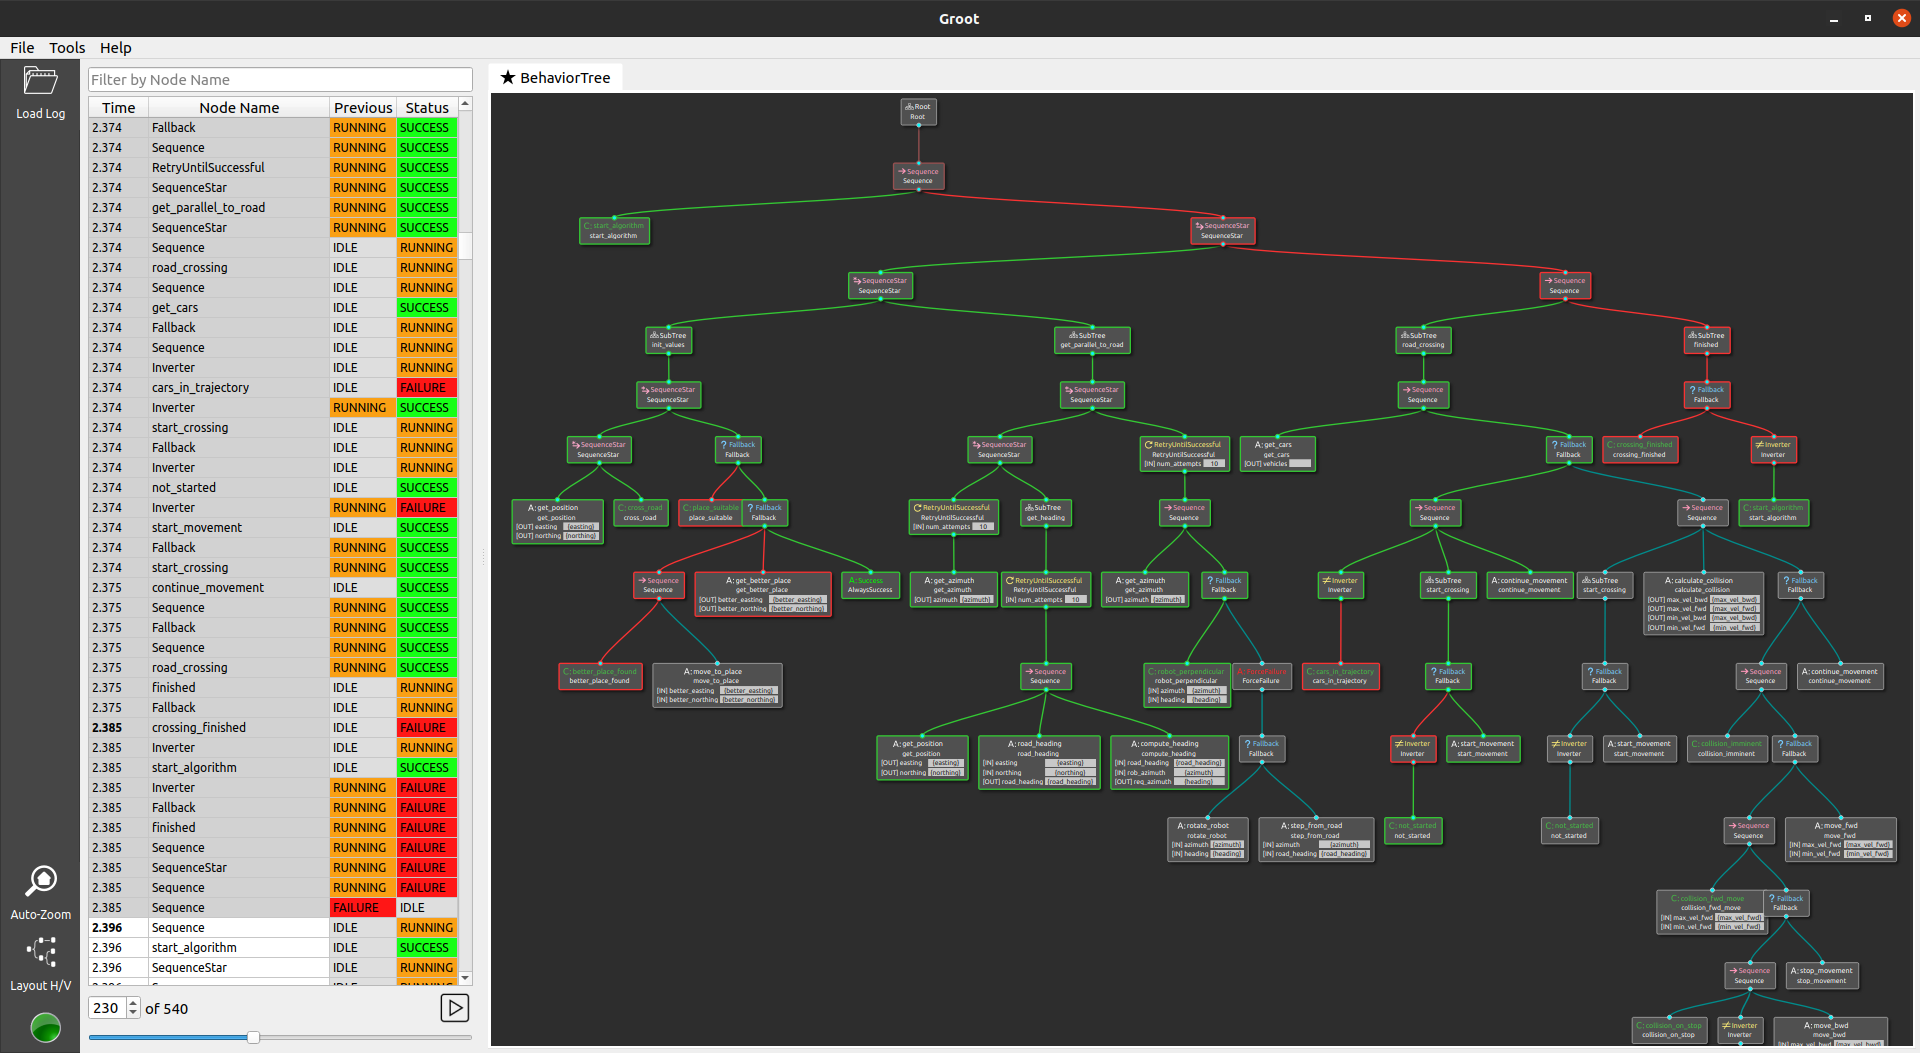
\includegraphics[width=\linewidth]{images/log_viewer.png}
        \caption{Log viewer in \texttt{Groot} application.}
        \label{fig:log_viewer}
    \end{figure}
\section{Algorithm behavior experiments}
    Once the stability of our algorithm was verified, we proceeded to test its behavior in different scenarios. We created several settings, each with a different configuration of the environment. With these scenarios, we tested the optimality and universality of our algorithm.\\
    We will present a few of the scenarios we created and discuss the results of the experiments and their importance within the validation process.\\
    We will present multiple figures with the settings of the vehicles relative to the robot. All used units correspond to the ones defined in section \ref{sec:Crossing-BT-impl}. The distances between objects in overviews are relative, not absolute. Also, if acceleration is not specified, it is assumed to be zero.\\
    \subsection{Used metrics}
    \label{sec:metrics}
        One of our tasks in the thesis assignment was to propose a metric for measuring the optimality of the robot's movement. The metric we created and used for evaluation is presented in this section.\\
        With each simulation experiment, we will present two graphs. One graph will show the minimal distance between the bounding boxes of the robot and the vehicle. The second graph will show the velocities of the vehicles and the robot during its movement.\\
        The minimal distance between the bounding boxes of the robot and the vehicle is a good metric for measuring the safety of the robot's movement. The smaller the distance, the higher the risk of collision.\\
        The velocities of the robot are also a good metric for measuring the optimality of the robot's movement. The higher the velocity, the faster the robot will reach its goal.\\
        Other useful metrics for measuring the optimality of the robot's movement are the time it would take the robot to cross the road should it be empty and the time it took to cross the road in the given scenario. Another parameter is whether the robot was able to cross the road. And lastly, the minimal and average time to collision and the difference from start time to collision.\\
        The time to collision represents the estimated duration it would take for the robot to collide with the vehicle, assuming the robot maintains its current trajectory while the vehicle comes to a stop. The average time will be calculated from all relevant measurements. It would be pointless to calculate the time of collision if such collision is not possible.\\
        The deviation from the initial time to collision refers to the amount of time the robot would need to adjust the start time of its movement to ensure a collision occurs.
    \subsection{Simulation scenarios and results}
        In most of the scenarios, we have tested certain behavior patterns. However, evaluation of algorithm robustness is also necessary. In some scenarios, there are one or more detection imprecisions or false detections altogether. The main scenario in which we verified robustness was scenario 5.\\\\
        \bfc{Scenario 1}\\
            The environment of the first scenario is shown in figure \ref{fig:scene1}. This simulation aims to test the algorithm's capabilities of calculating the optimal velocities for the robot. As this was our first proper experiment, the condition node determining if the road was crossed was also tested.\\
            \begin{figure}[H]
                \centering
                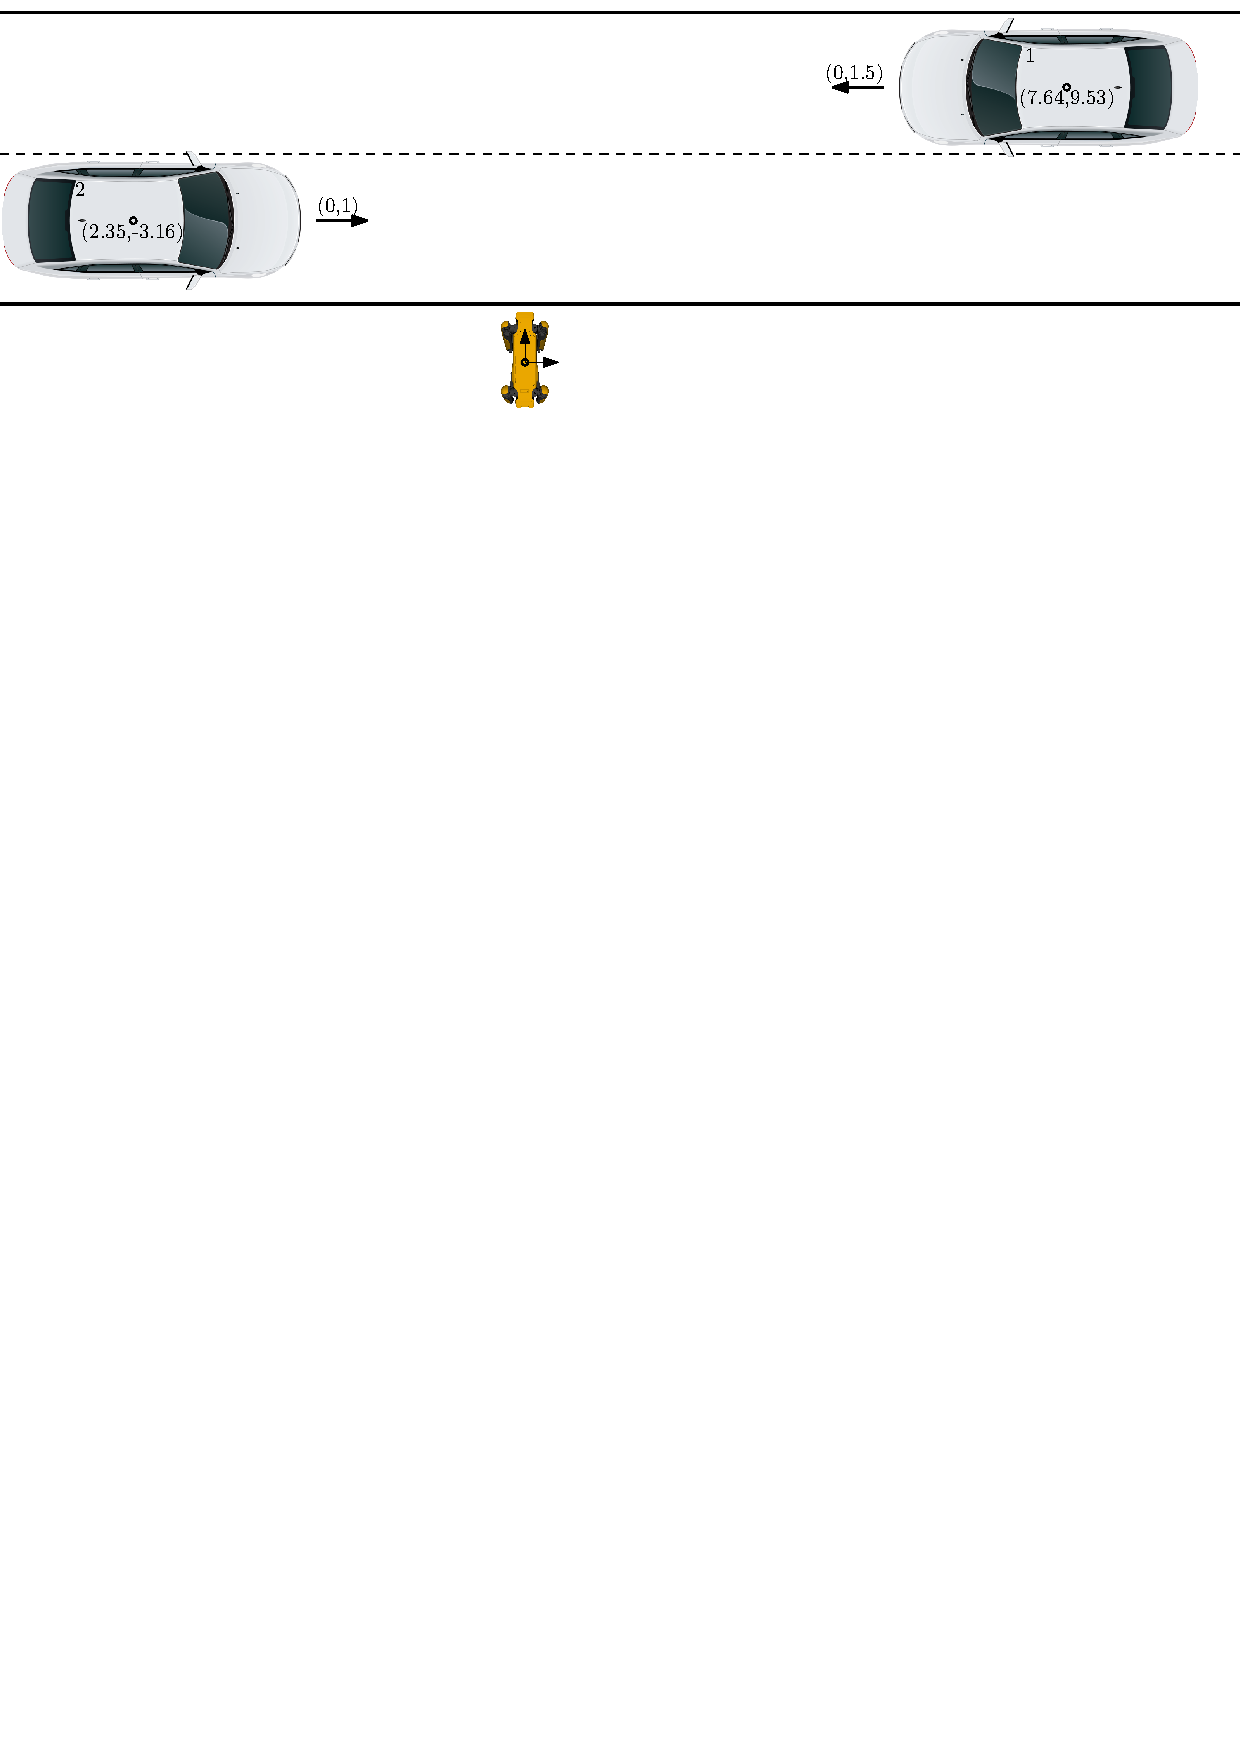
\includegraphics[width=0.95\linewidth]{images/simulations/scene1.pdf}
                \caption{Environment for the first simulation scenario.}
                \label{fig:scene1}
            \end{figure}
            The graphs detailing the results of the experiment are shown in figure \ref{fig:scene1_graphs}.
            \begin{figure}[H]
                \centering
                \begin{subfigure}{0.49\linewidth}
                    \centering
                    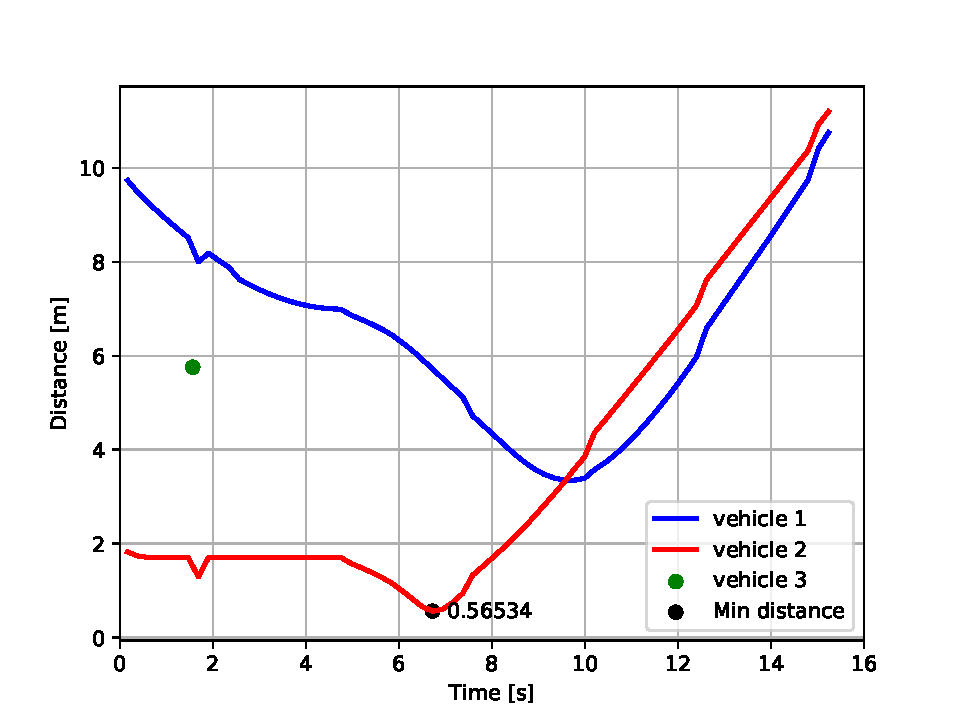
\includegraphics[trim={13 8 40 41}, clip, width=\linewidth]{images/simulations/scene1_dist.pdf}
                    \caption{Minimal distance between the robot and detected vehicles.}
                \end{subfigure}
                \begin{subfigure}{0.49\linewidth}
                    \centering
                    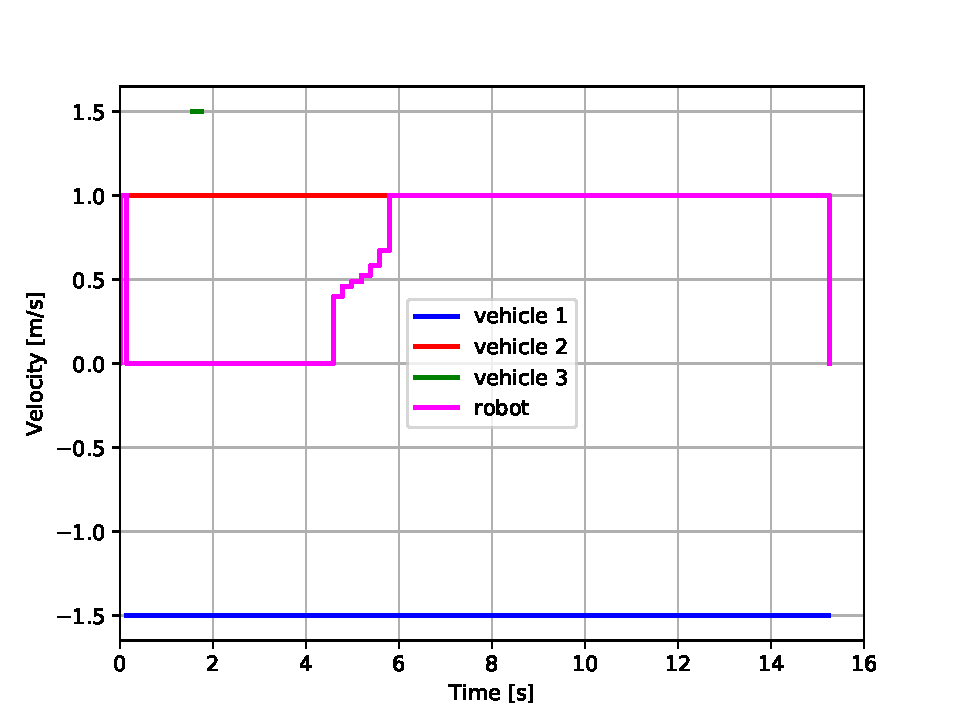
\includegraphics[trim={13 8 40 41}, clip, width=\linewidth]{images/simulations/scene1_vel.pdf}
                    \caption{Velocities of the robot and vehicles during the crossing.}
                \end{subfigure}
                \caption{Results for the first scenario of simulation experiments.}
                \label{fig:scene1_graphs}
            \end{figure}
        \bfc{Scenario 2}\\
            In the second scenario, we used the configuration shown in figure \ref{fig:scene2}. This scenario was used to test our algorithm's prediction of the vehicle's trajectory. We constructed three further sub-scenarios. Firstly, the deceleration of the vehicle would stop the vehicle in the path of the robot. Secondly, the vehicle would come to a stop after crossing the robot's path. Lastly, with the highest deceleration, the vehicle would stop before crossing the robot's path.\\
            \begin{figure}[H]
                \centering
                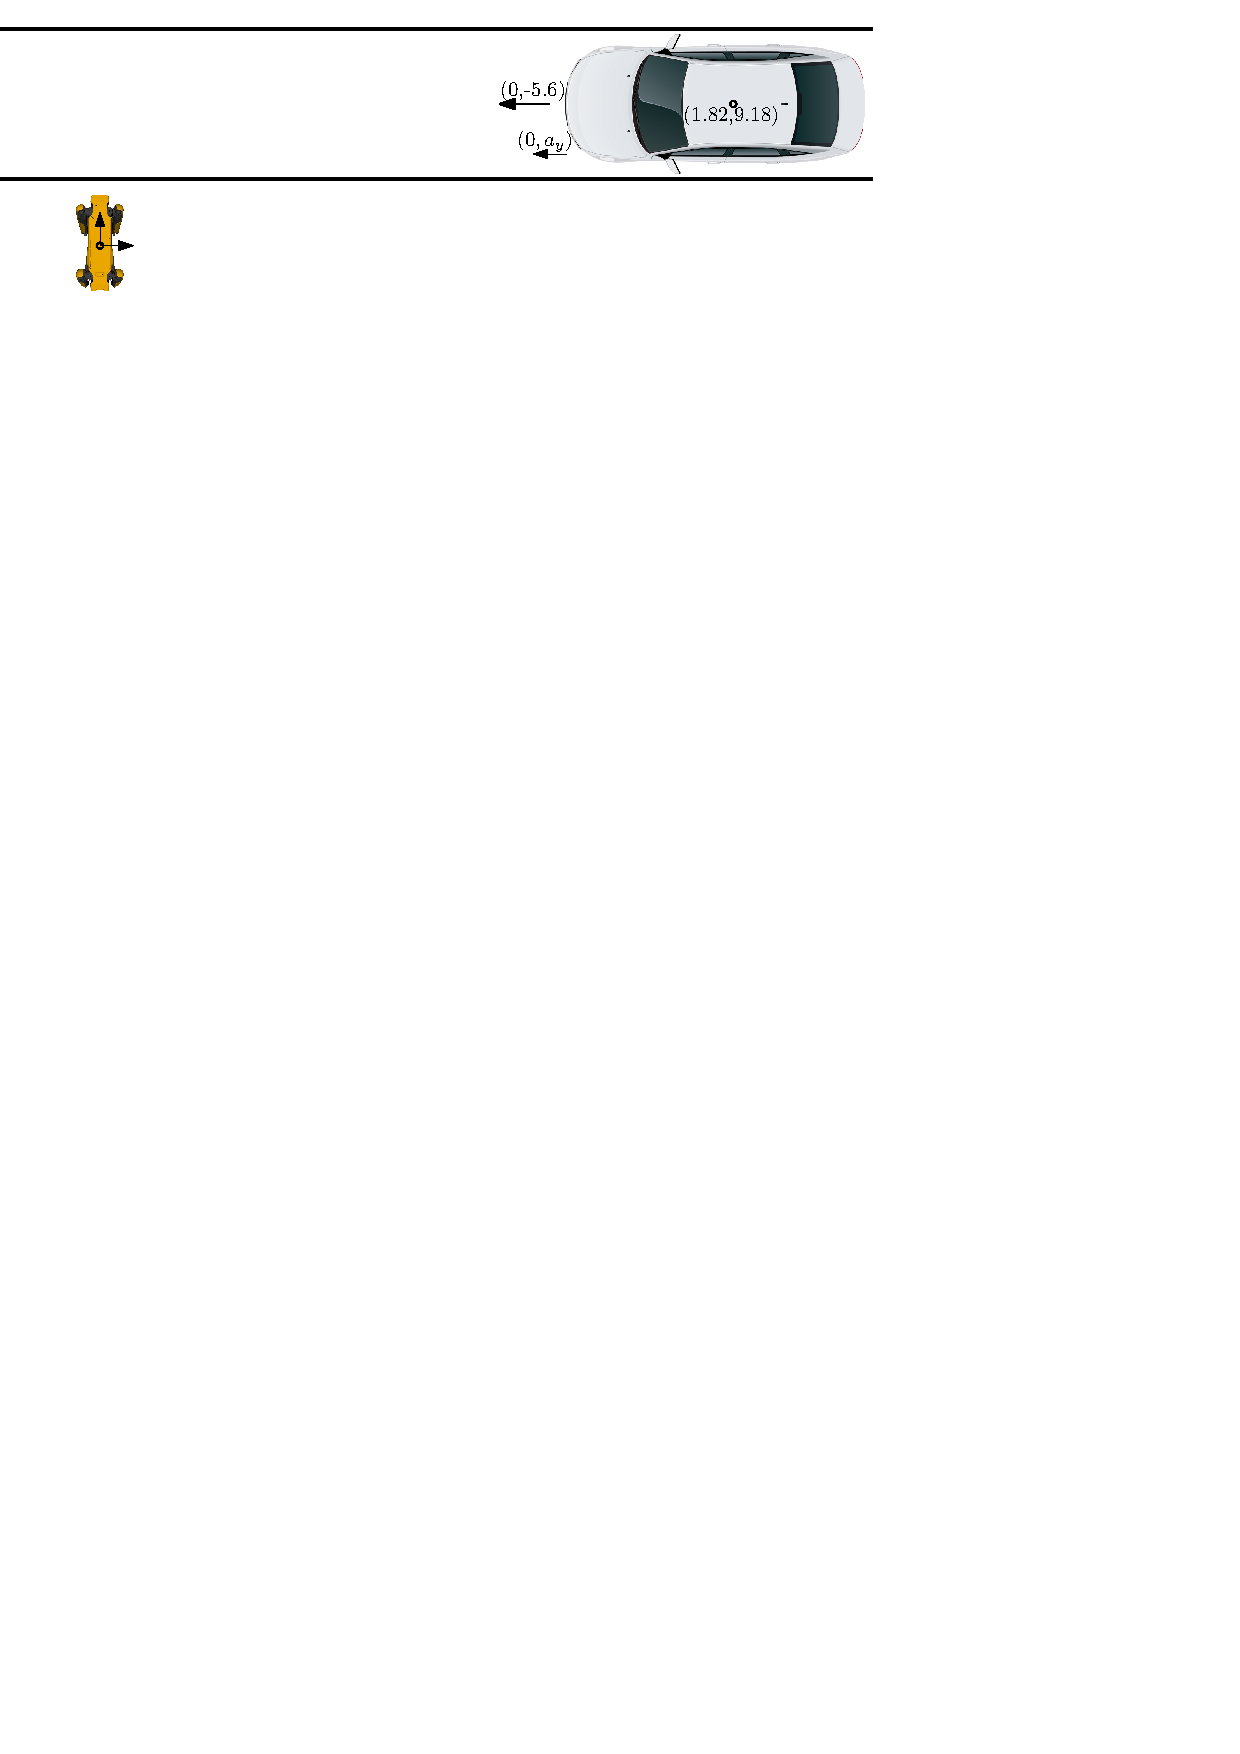
\includegraphics[width=0.95\linewidth]{images/simulations/scene2.pdf}
                \caption{Environment for the second simulation scenario.}
                \label{fig:scene2}
            \end{figure}
            The results of the first sub-scenario are shown in \ref{fig:scene2_1_graphs}, the second sub-scenario in \ref{fig:scene2_2_graphs}, and the third sub-scenario in \ref{fig:scene2_3_graphs}.
            \begin{figure}[H]
                \centering
                \begin{subfigure}{0.49\linewidth}
                    \centering
                    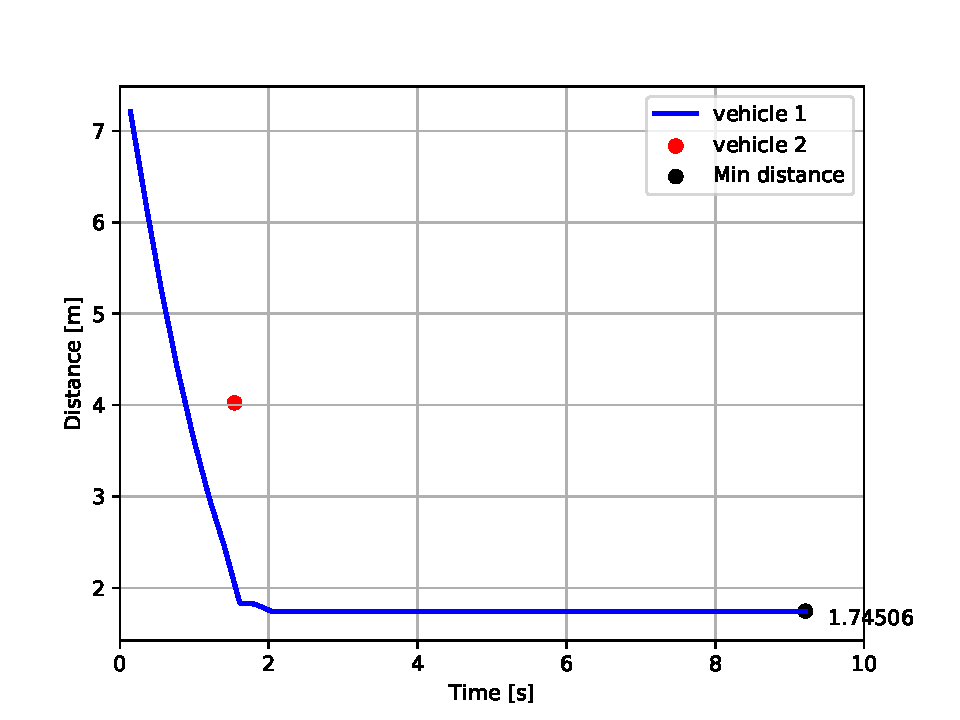
\includegraphics[trim={24 8 35 41}, clip, width=\linewidth]{images/simulations/scene2_1_dist.pdf}
                    \caption{Minimal distance between the robot and detected vehicles.}
                \end{subfigure}
                \begin{subfigure}{0.49\linewidth}
                    \centering
                    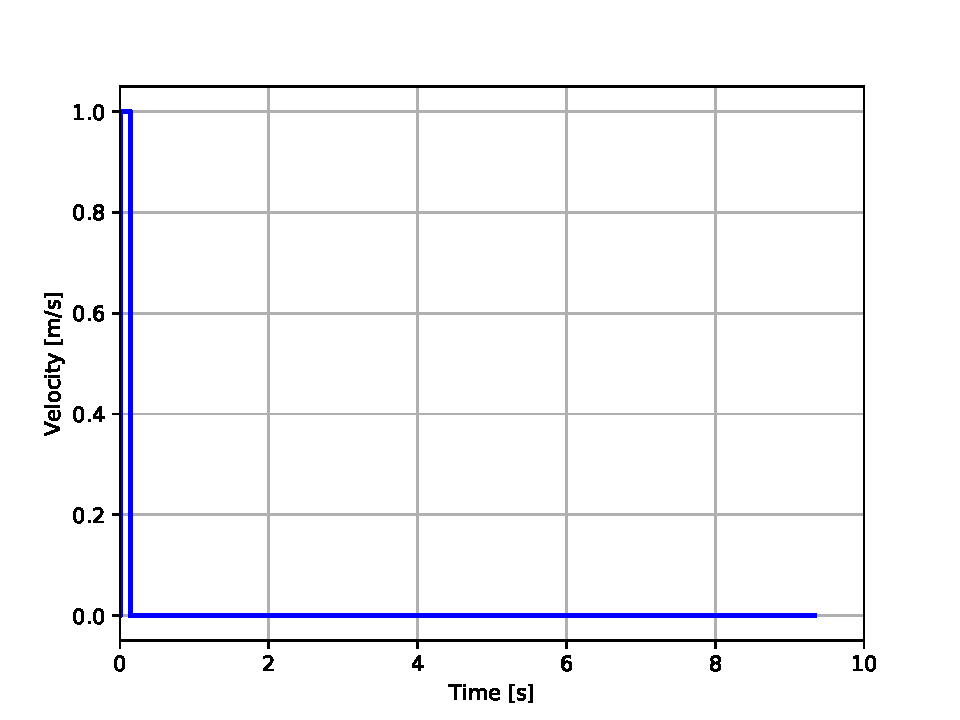
\includegraphics[trim={21 8 40 41}, clip, width=\linewidth]{images/simulations/scene2_1_vel.pdf}
                    \caption{Velocities of the robot and vehicles during the crossing.}
                \end{subfigure}
                \caption{Results for the first sub-scenario in the second scenario of simulations.}
                \label{fig:scene2_1_graphs}
            \end{figure}
            \begin{figure}[H]
                \centering
                \begin{subfigure}{0.49\linewidth}
                    \centering
                    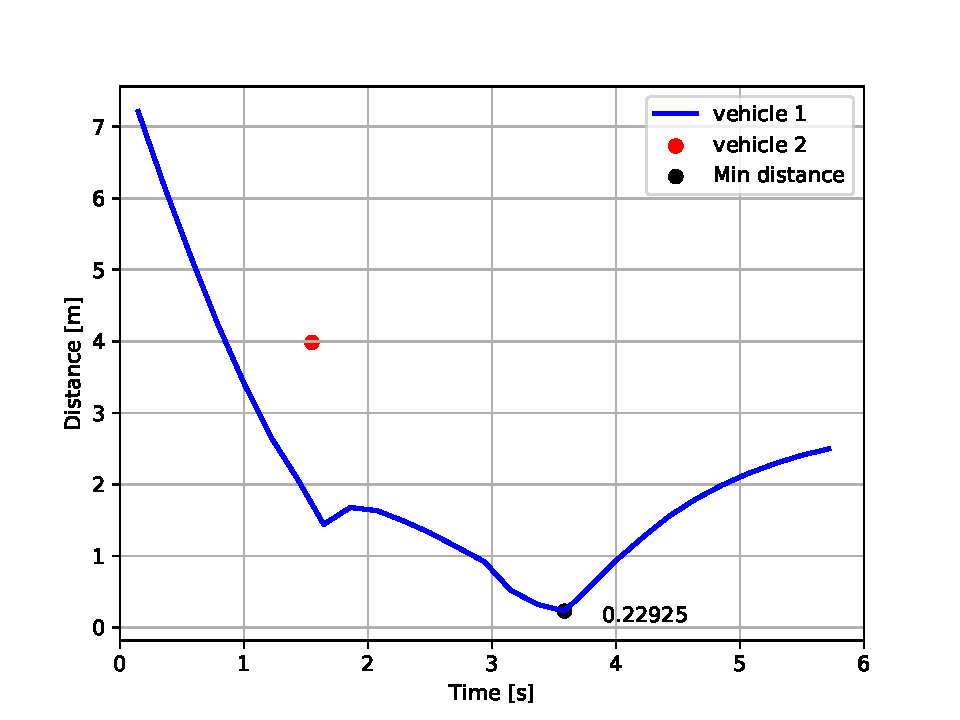
\includegraphics[trim={24 8 40 41}, clip, width=\linewidth]{images/simulations/scene2_2_dist.pdf}
                    \caption{Minimal distance between the robot and detected vehicles.}
                \end{subfigure}
                \begin{subfigure}{0.49\linewidth}
                    \centering
                    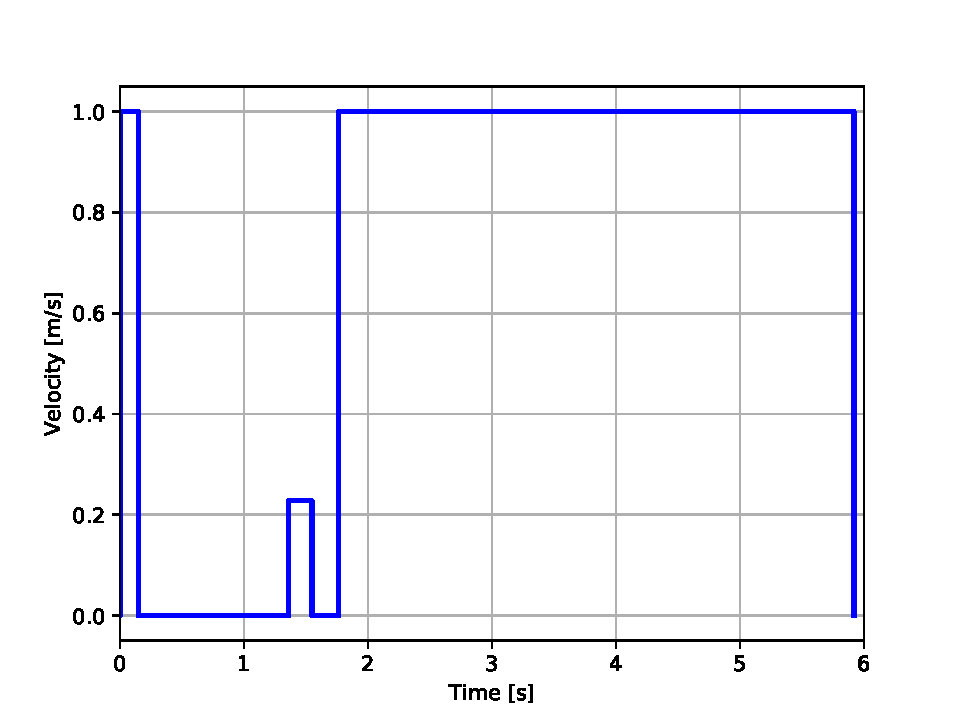
\includegraphics[trim={21 8 40 41}, clip, width=\linewidth]{images/simulations/scene2_2_vel.pdf}
                    \caption{Velocities of the robot and vehicles during the crossing.}
                \end{subfigure}
                \caption{Results for the second sub-scenario in the second scenario of simulations.}
                \label{fig:scene2_2_graphs}
            \end{figure}
            \begin{figure}[H]
                \centering
                \begin{subfigure}{0.49\linewidth}
                    \centering
                    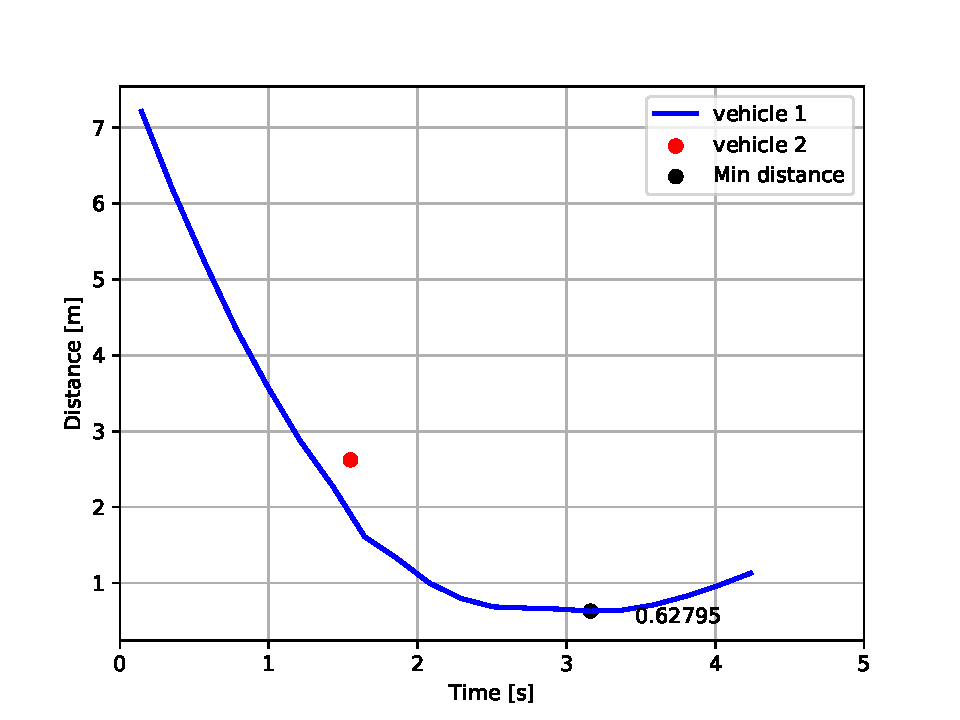
\includegraphics[trim={24 8 40 41}, clip, width=\linewidth]{images/simulations/scene2_3_dist.pdf}
                    \caption{Minimal distance between the robot and detected vehicles.}
                \end{subfigure}
                \begin{subfigure}{0.49\linewidth}
                    \centering
                    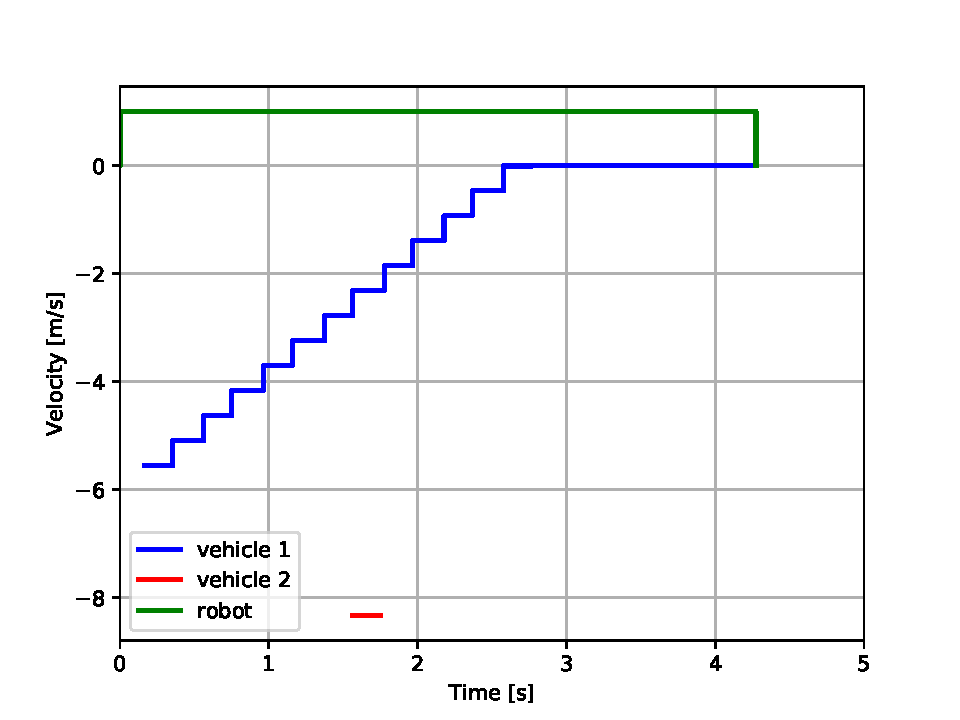
\includegraphics[trim={21 8 40 41}, clip, width=\linewidth]{images/simulations/scene2_3_vel.pdf}
                    \caption{Velocities of the robot and vehicles during the crossing.}
                \end{subfigure}
                \caption{Results for the third sub-scenario in the second scenario of simulations.}
                \label{fig:scene2_3_graphs}
            \end{figure}
        \bfc{Scenario 3}\\
            With this simulation experiment, we wanted to validate the algorithm's ability to handle multiple vehicles in a line. In this simulation, the vehicles also started from a greater distance and moved with greater velocities. The environment of the simulation is shown in figure \ref{fig:scene3}.\\
            \begin{figure}[H]
                \centering
                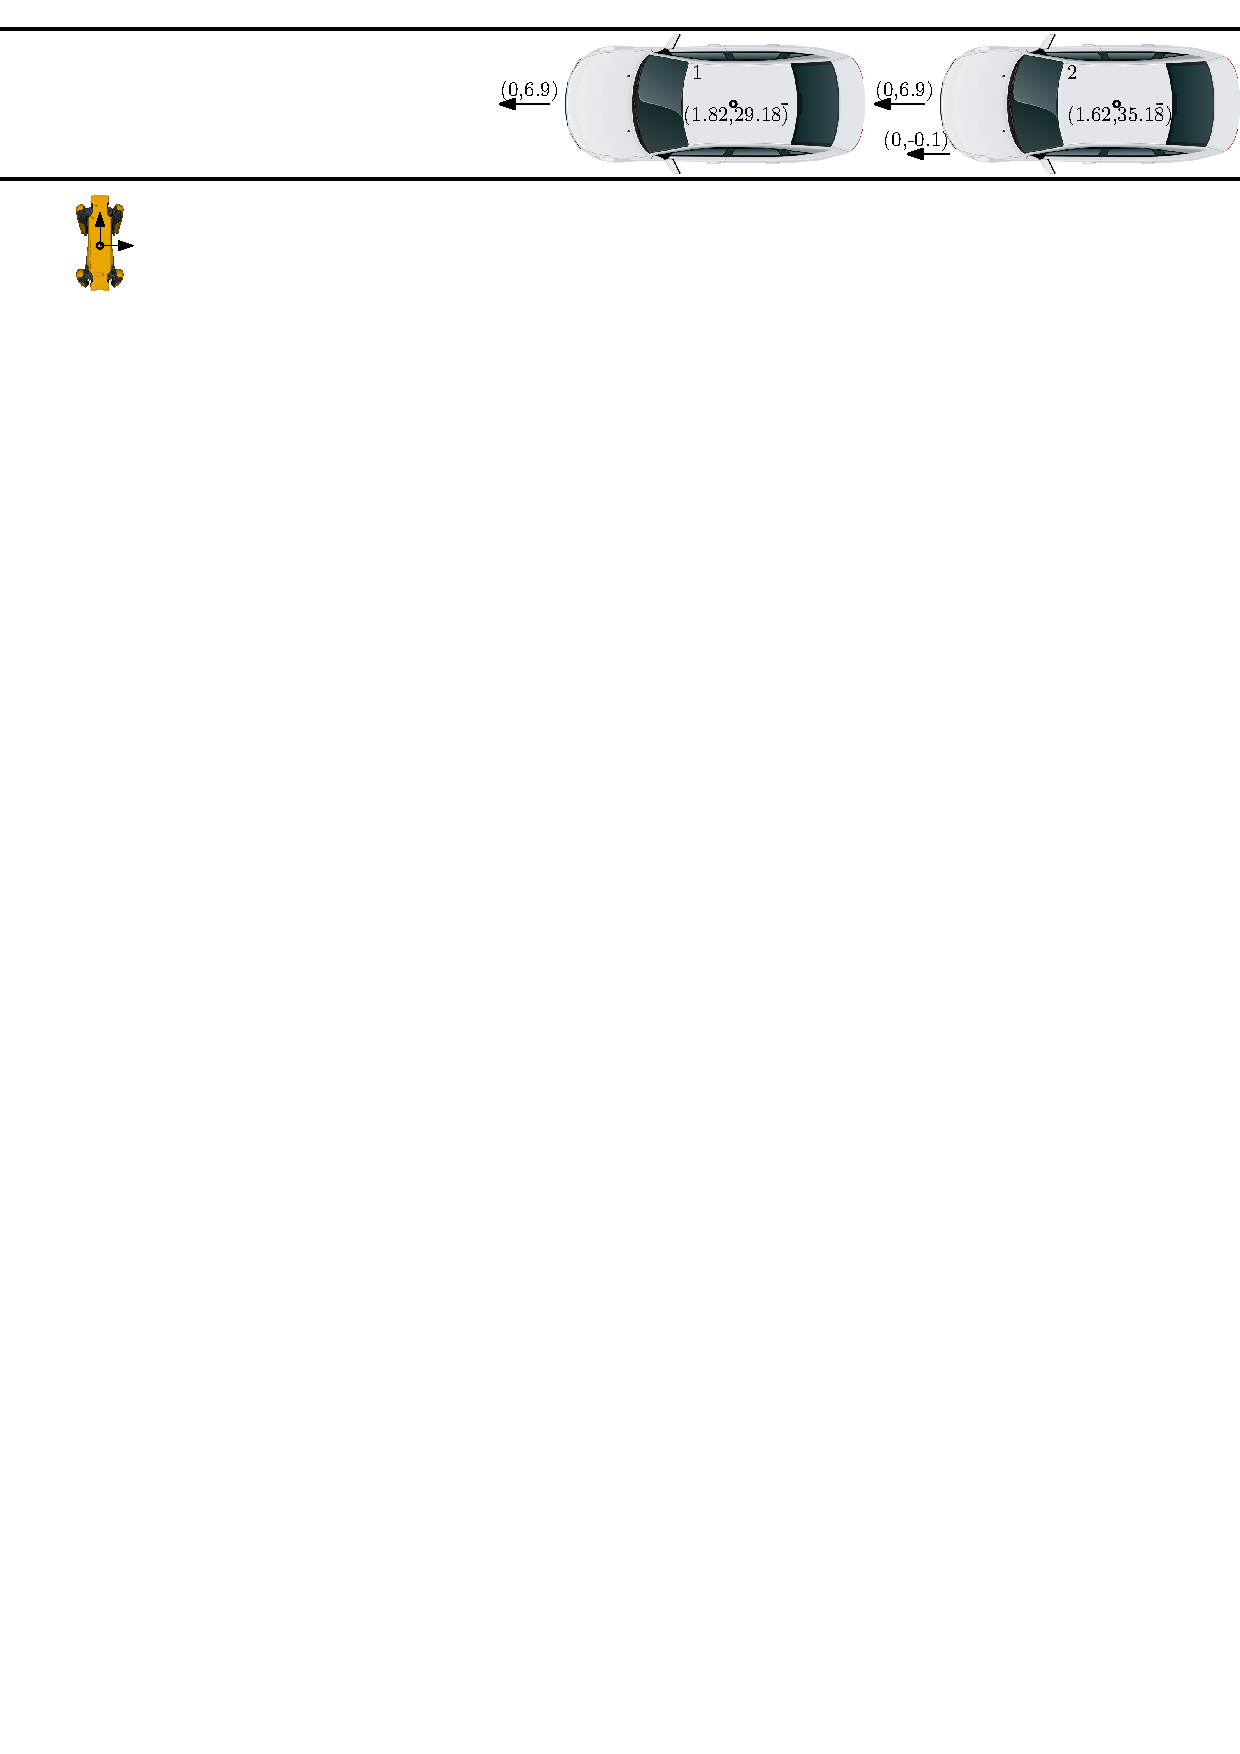
\includegraphics[width=0.95\linewidth]{images/simulations/scene3.pdf}
                \caption{Environment for the third simulation scenario.}
                \label{fig:scene3}
            \end{figure}
            The results are shown in graphs \ref{fig:scene3_graph1} and \ref{fig:scene3_graph2}.
            \begin{figure}[H]
                \centering
                \begin{subfigure}{0.49\linewidth}
                    \centering
                    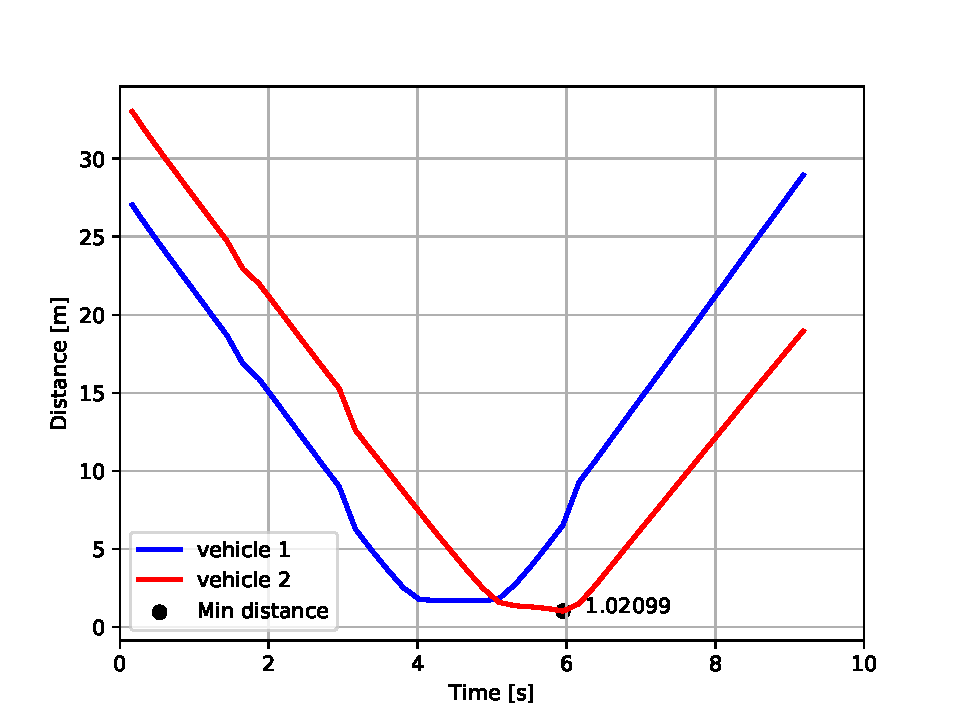
\includegraphics[trim={24 8 40 41}, clip, width=\linewidth]{images/simulations/scene3_dist.pdf}
                    \caption{Minimal distance between the robot and vehicles.}
                    \label{fig:scene3_graph1}
                \end{subfigure}
                \begin{subfigure}{0.49\linewidth}
                    \centering
                    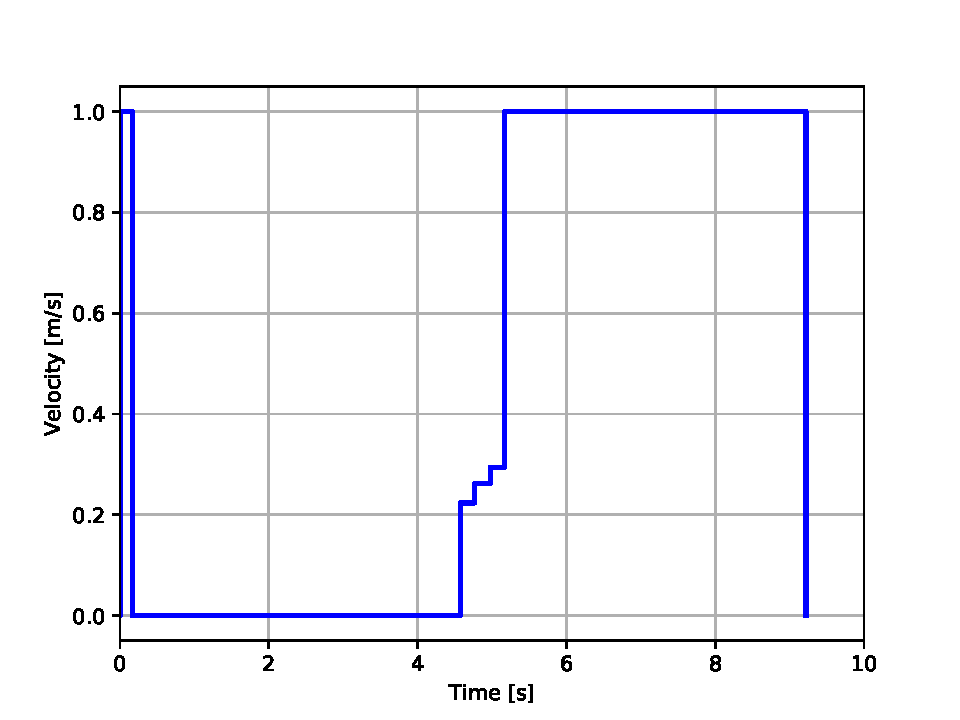
\includegraphics[trim={21 8 40 41}, clip, width=\linewidth]{images/simulations/scene3_vel.pdf}
                    \caption{Velocities of the robot and vehicles during the crossing.}
                    \label{fig:scene3_graph2}
                \end{subfigure}
                \caption{Results for the third scenario of simulation experiments.}
                \label{fig:scene3_graphs}
            \end{figure}
        \bfc{Scenario 4}\\
            Figure \ref{fig:scene4} shows the setting for this simulation experiment. This experiment aimed to test the impact of the velocity margin on the robot's behavior. The velocity margin is a set constant value, we want to keep the robot's velocity from the calculated velocity interval by this margin. This should ensure that the robot will keep some minimal distance from the vehicles. We ran two simulations, one with a velocity margin set to $0.15\:\si{\m\per\s}$ and the other with a velocity margin set to $0.25\:\si{\m\per\s}$. The results are shown in graphs \ref{fig:scene4_1_graphs} and \ref{fig:scene4_2_graphs}.\\
            \begin{figure}[H]
                \centering
                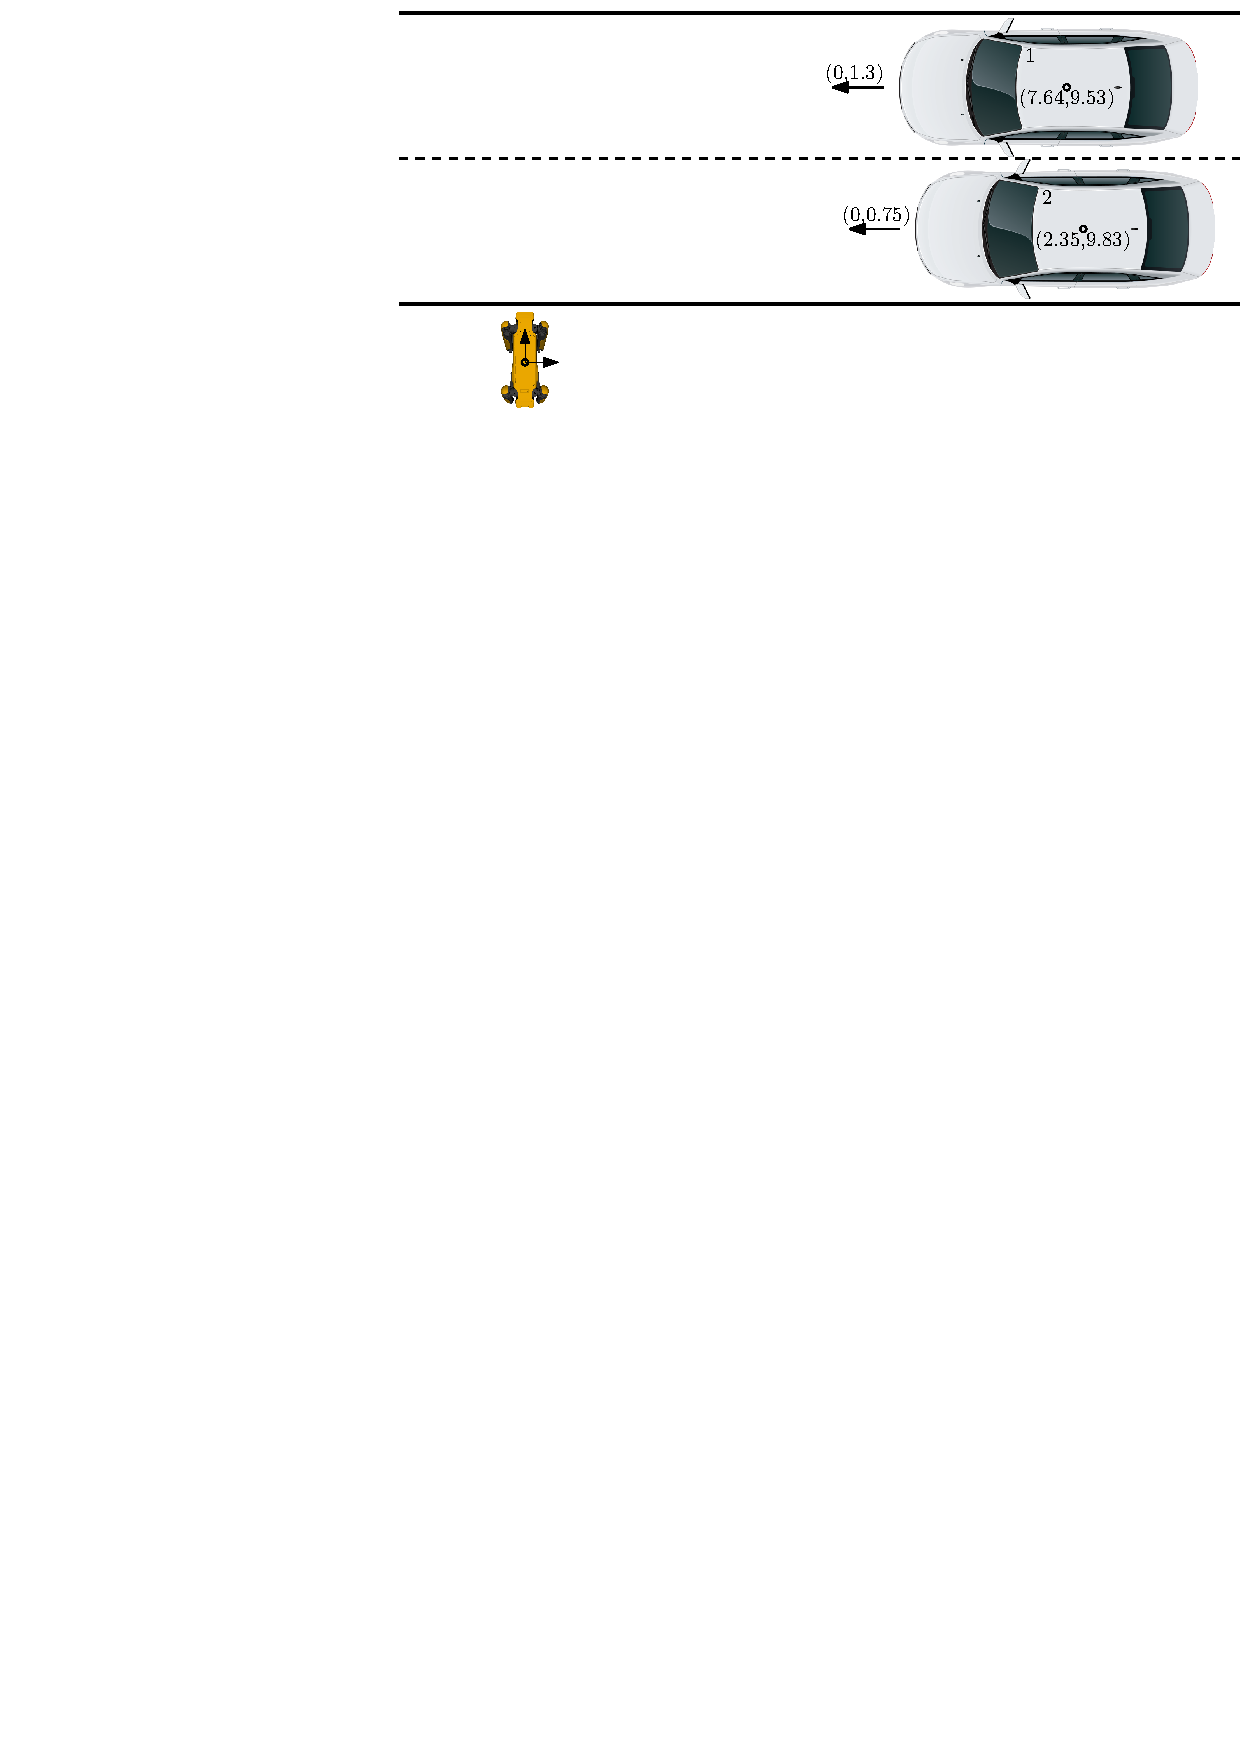
\includegraphics[width=0.95\linewidth]{images/simulations/scene4.pdf}
                \caption{Environment for the fourth simulation scenario.}
                \label{fig:scene4}
            \end{figure}
            By comparing the two runs, it becomes evident that in the second simulation run, with a larger safety margin, the robot waited for both vehicles to pass before crossing. On the contrary, in the first run, the robot decided to cross the road in front of the closer vehicle.\\
            \begin{figure}[H]
                \centering
                \begin{subfigure}{0.49\linewidth}
                    \centering
                    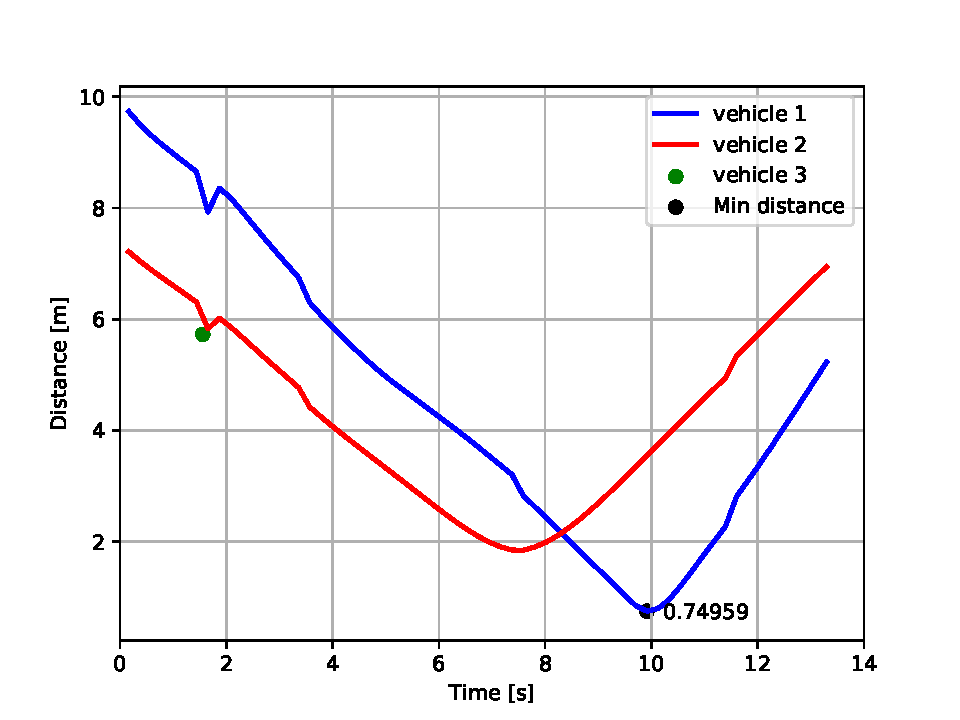
\includegraphics[trim={13 8 40 41}, clip, width=\linewidth]{images/simulations/scene4_1_dist.pdf}
                    \caption{Minimal distance between the robot and vehicles.}
                \end{subfigure}
                \begin{subfigure}{0.49\linewidth}
                    \centering
                    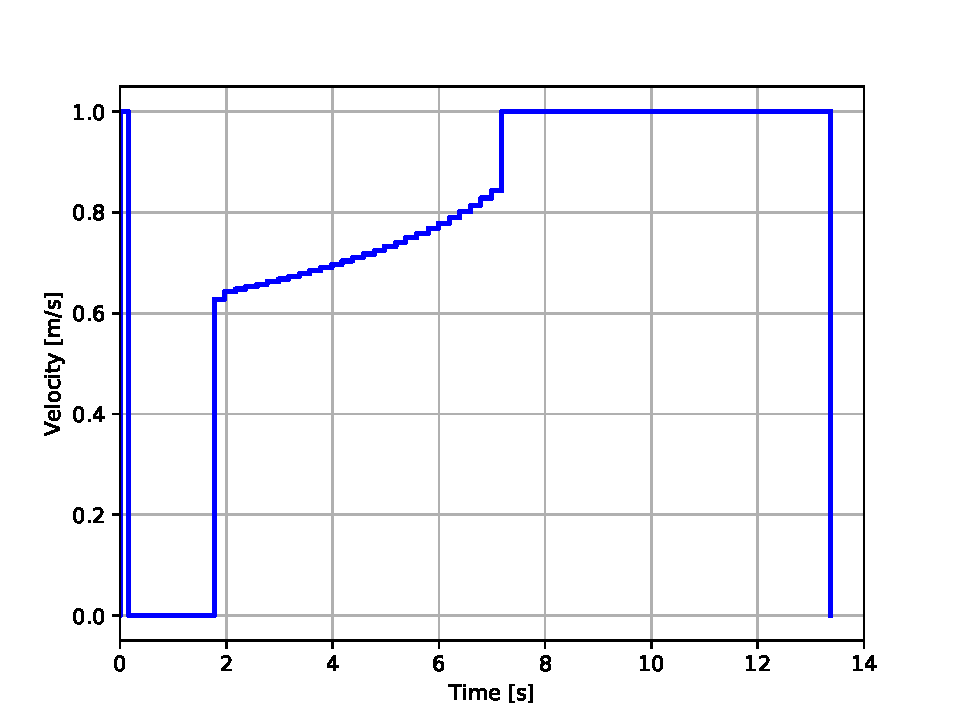
\includegraphics[trim={13 8 40 41}, clip, width=\linewidth]{images/simulations/scene4_1_vel.pdf}
                    \caption{Velocities of the robot and vehicles during the crossing.}
                \end{subfigure}
                \caption{Results for the first run of the fourth scenario of simulation experiments.}
                \label{fig:scene4_1_graphs}
            \end{figure}
            \begin{figure}[H]
                \centering
                \begin{subfigure}{0.49\linewidth}
                    \centering
                    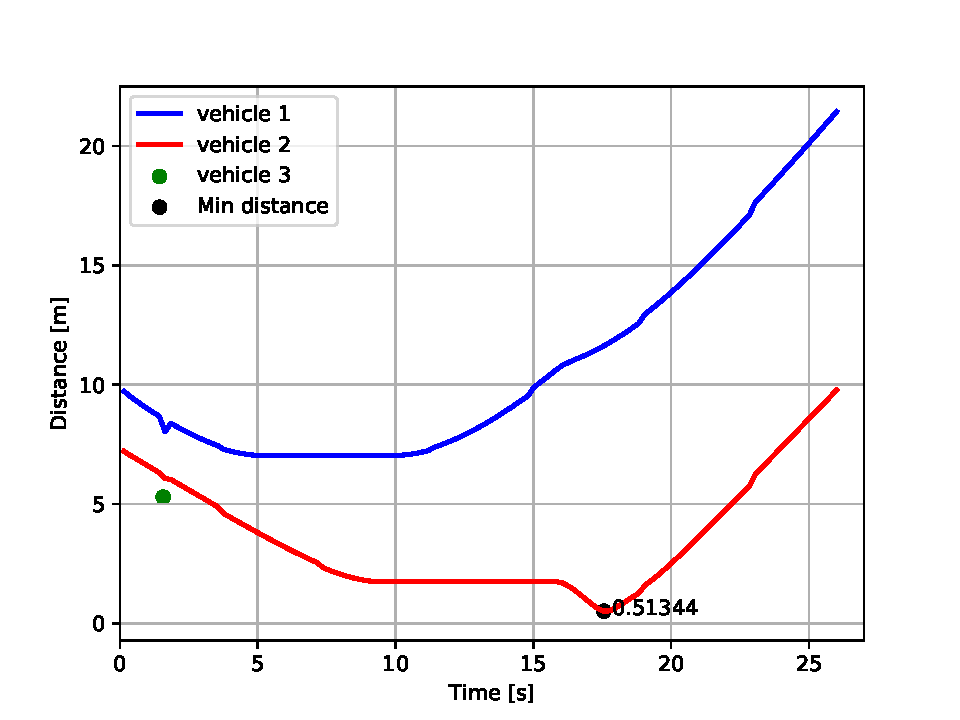
\includegraphics[trim={13 8 40 41}, clip, width=\linewidth]{images/simulations/scene4_2_dist.pdf}
                    \caption{Minimal distance between the robot and vehicles.}
                \end{subfigure}
                \begin{subfigure}{0.49\linewidth}
                    \centering
                    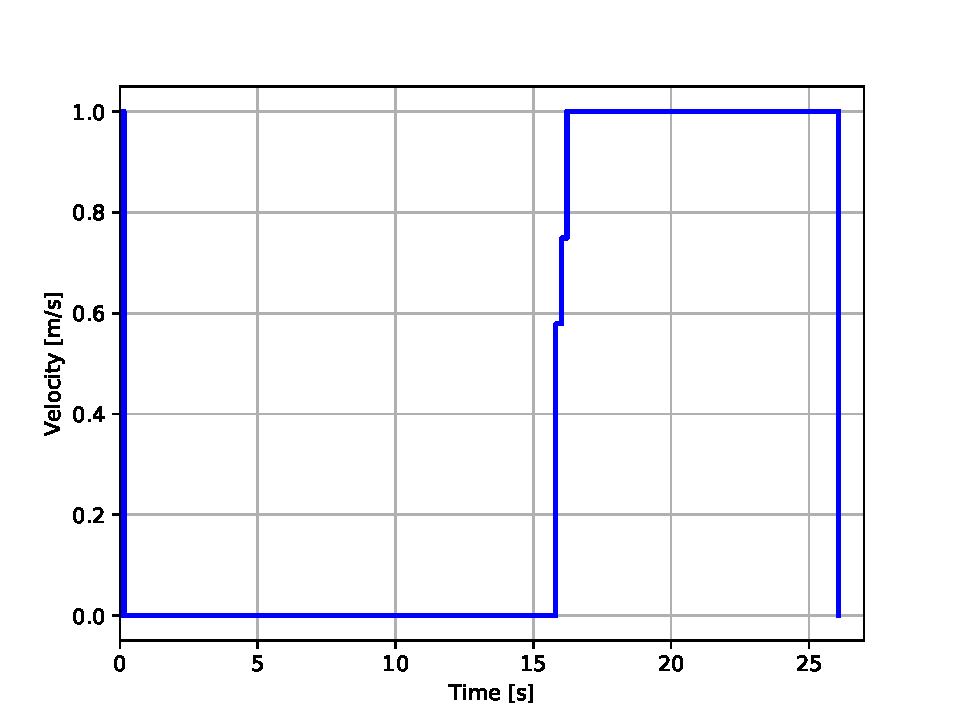
\includegraphics[trim={13 8 40 41}, clip, width=\linewidth]{images/simulations/scene4_2_vel.pdf}
                    \caption{Velocities of the robot and vehicles during the crossing.}
                \end{subfigure}
                \caption{Results for the second run of the fourth scenario of simulation experiments.}
                \label{fig:scene4_2_graphs}
            \end{figure}
        \bfc{Scenario 5}\\
            The last simulation experiment aimed to evaluate and test the robustness of our algorithm. We run multiple iterations of the same configuration, each with detection imprecisions. As these imprecisions are generated randomly, we obtained a more comprehensive insight into the algorithm's robustness. The environment of the simulation is shown in figure \ref{fig:scene5}.\\
            \begin{figure}[H]
                \centering
                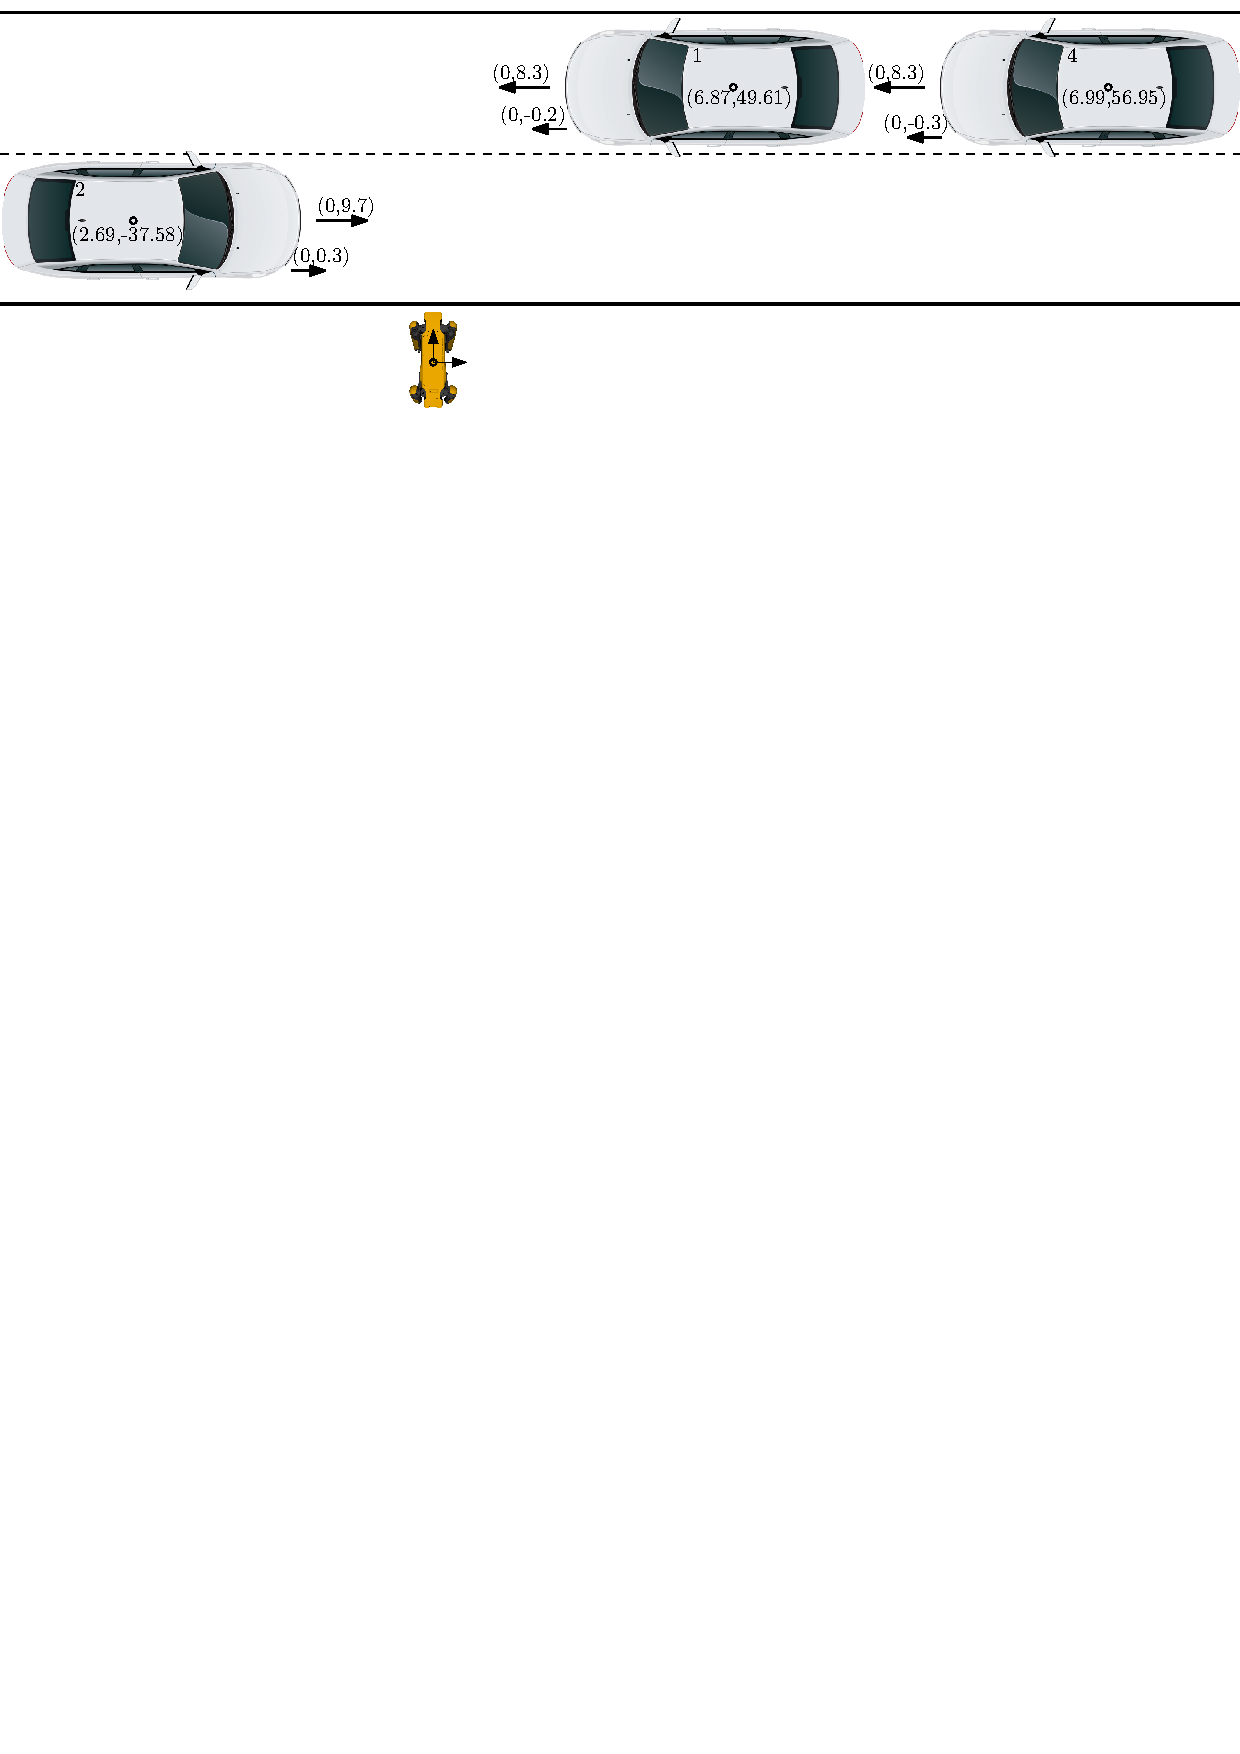
\includegraphics[width=0.95\linewidth]{images/simulations/scene5.pdf}
                \caption{Environment for the fifth simulation scenario.}
                \label{fig:scene5}
            \end{figure}
            The results of one of the runs are shown in graphs \ref{fig:scene5_graphs}. The graph \ref{fig:scene5_vel} shows that the robot would move in a jerking motion. While a smoothing filter could be implemented, we opted not to do so, as it would remove the robot's ability to escape danger quickly.\\
            The effect of imprecise detection is quite evident on the lines detailing the minimal distance between vehicles and the robot. This graph was constructed from the detected positions and not from the actual position of the vehicles. Even though it does not provide us with the safety aspect of the robot's behavior, it gives an insight into the algorithm's decision-making. The difference between the actual and detected position is also not so significant to render this data unusable for the discussion of safety.\\
            \begin{figure}[H]
                \centering
                \begin{subfigure}{0.49\linewidth}
                    \centering
                    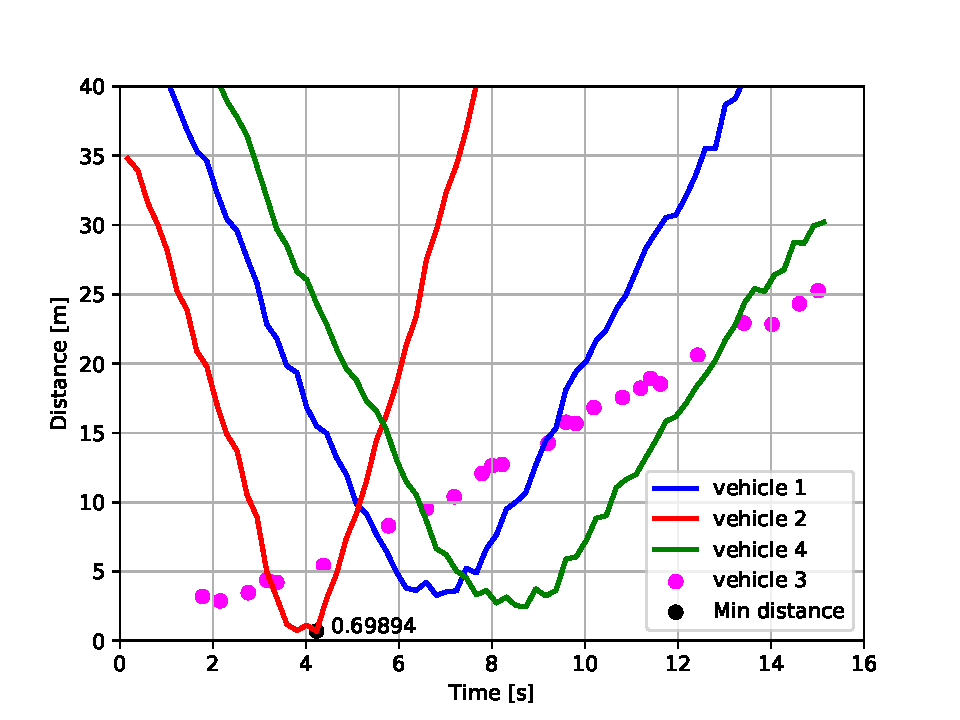
\includegraphics[trim={24 8 40 37}, clip, width=\linewidth]{images/simulations/scene5_dist.pdf}
                    \caption{Minimal distance between the robot and vehicles.}
                \end{subfigure}
                \begin{subfigure}{0.49\linewidth}
                    \centering
                    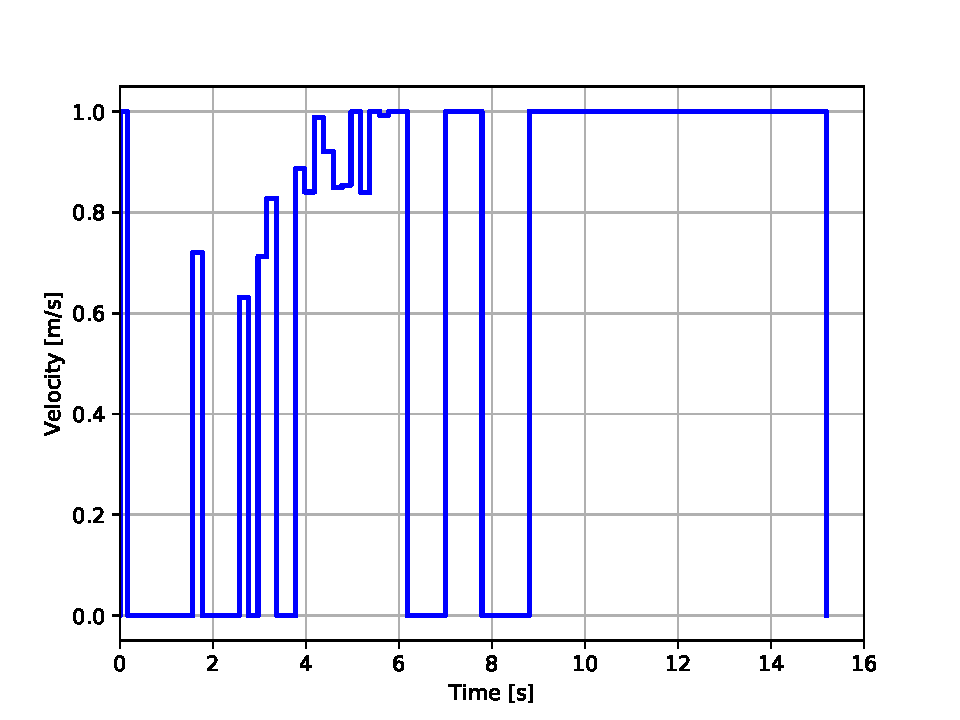
\includegraphics[trim={21 8 40 37}, clip, width=\linewidth]{images/simulations/scene5_vel.pdf}
                    \caption{Velocities of the robot and vehicles during the crossing.}
                    \label{fig:scene5_vel}
                \end{subfigure}
                \caption{Results for the fifth scenario of simulation experiments.}
                \label{fig:scene5_graphs}
            \end{figure}
    \subsection{Evaluation of the results}
        In this section, we will discuss the results of the simulation experiments. We will use the metric proposed in section \ref{sec:metrics}.\\
        From the distance graphs, we can see that the robot was able to maintain a safe distance from the vehicles. The minimal distance, shown in table \ref{tab:dist}, was never smaller than $0.5\:\si{\m}$, and most of these minimal distances were achieved after the vehicle crossed the robot's path. Therefore, there was no danger of collision even if the vehicle performed some unexpected maneuver.\\
        \begin{table}[H]
            \centering
            \begin{tabular}{|c||c|c|c|c|c|c|c|c|}
                \hline
                Scenario & 1 & 2.1 & 2.2 & 2.3 & 3 & 4.1 & 4.2 & 5 \\
                \hline
                Minimal distance $[\si{\m}]$ & 0.54 & 1.74 & 1.00 & 0.63 & 1.01 & 0.74 & 0.52 & 0.85 \\
                \hline
            \end{tabular}
            \caption{Minimal distance between the robot and vehicles in the simulation experiments.}
            \label{tab:dist}
        \end{table}
        Another two parameters of the metric are the ratio of time it would take to cross the empty road to the time of the crossing in the simulated environment and whether the robot crossed the road. The time ratio is calculated with the following equation
        \begin{equation}
            \Delta t = \frac{t_{\text{simulated}}}{t_{\text{empty}}}
        \end{equation}
        \noindent These two parameters are shown in table \ref{tab:met1}.
        \begin{table}[H]
            \centering
            \begin{tabular}{|c||c|c|c|c|c|c|c|c|}
                \hline
                Scenario & 1 & 2.1 & 2.2 & 2.3 & 3 & 4.1 & 4.2 & 5 \\
                \hline
                Time ratio $\Delta t$ & 1.53 & \emph{NA} & 1.71 & 1.07 & 2.36 & 1.34 & 2.61 & 1.35 \\
                \hline
                Crossed & Yes & No & Yes & Yes & Yes & Yes & Yes & Yes \\
                \hline
            \end{tabular}
            \caption{Simulation experiment results showing the time ratio and successful crossing parameters of the metric.}
            \label{tab:met1}
        \end{table}
        \noindent In all except one scenario, the robot was able to finish the crossing. However, scenario 2.1 was specifically designed for the robot not to be able to cross the road. It is also evident that the $\Delta t$ is highly relative as this parameter depends on the traffic and the velocity margin gap we imposed on the robot.\\
        Table \ref{tab:times} shows the metric's last two parameters.
        \begin{table}[H]
            \centering
            \begin{tabular}{|c|c c|c|}
                \hline
                \multirow{2}{4em}{Scenario} & \multicolumn{2}{c|}{Time to contact [$\si{\s}$]} & \multirow{2}{9em}{Start time change [$\si{\s}$]}\\
                & Average & Minimal & \\
                \hline\hline
                \multicolumn{1}{|l|}{Scenario 1} & $6.36$ & $1.16$ & $-6.38,\ -4.22$ \\
                \hline
                Scenario 2.1 & \emph{NA} & \emph{NA} & \emph{NA} \\
                \hline
                Scenario 2.2 & $4.28$ & $1.14$ & $-3.15$ \\
                \hline
                Scenario 2.3 & \emph{NA} & \emph{NA} & \emph{NA} \\
                \hline
                \multicolumn{1}{|l|}{Scenario 3} & $4.46$ & $1.47$ & $-3.46,\ -2.55$ \\
                \hline
                Scenario 4.1 & $3.41$ & $1.24$ & $-3.65,\ 7.99$ \\
                \hline
                Scenario 4.2 & $1.96$ & $1.17$ & $-16.45,\ -5.27$ \\
                \hline
                \multicolumn{1}{|l|}{Scenario 5} & $2.72$ & $0.88$ & $-4.94,\ -2.51,\ -4.49$ \\
                \hline
            \end{tabular}
            \caption{Calculated values for time to contact and start time change for the simulation experiments.}
            \label{tab:times}
        \end{table}
        \noindent There are two scenarios where the answer is \emph{NA} (not answered). In scenario 2.1, the robot did not start moving, and in scenario 2.3, no vehicle crossed the robot's path. Calculating the result for either of these scenarios is nonsensical.\\
        The results for the time to contact indicate that the robot would be able to react and avoid a collision even in the case of an unexpected stop of the vehicle. The minimal values are all above $0.8\:\si{\s}$, and with the expected rate of detection node being $5\:\si{\Hz}$, it would have enough time to adapt. This is true even when we take into consideration the latency of obtaining the data from the detection node. We do not expect this latency to be higher than $0.2\:\si{\s}$, which would still provide about $0.4\:\si{\s}$ for the robot to react.\\
        Interpretation of the results for the start time change is straightforward. The robot starts moving at the time $t=0$. The negative values mean the robot must start earlier to collide, and the positive values indicate the robot must start later. The calculated times correspond to the velocities the robot had during the successful crossings. Each result in a scenario is associated with a specific vehicle, and their order is determined by their ID.
    \subsection{Interesting points from trajectories}
        We will show some interesting points from the trajectories of the movement of the robot and the vehicles. The parts we will show were when the robot began its movement, figure \ref{fig:start}, and got closest to the vehicle, figure \ref{fig:closest}. We will not show the starts in scenarios 2.1 and 2.3, as in scenario 2.1 the robot never began its movement, and in 2.3 it started immediately.\\
        The points shown as trajectories are the centers of the objects. In the vehicle trajectories, it is evident that most of the experiments contained a vehicle detection error. 
        \begin{figure}[H]
            \centering
            \begin{subfigure}{0.49\linewidth}
                \centering
                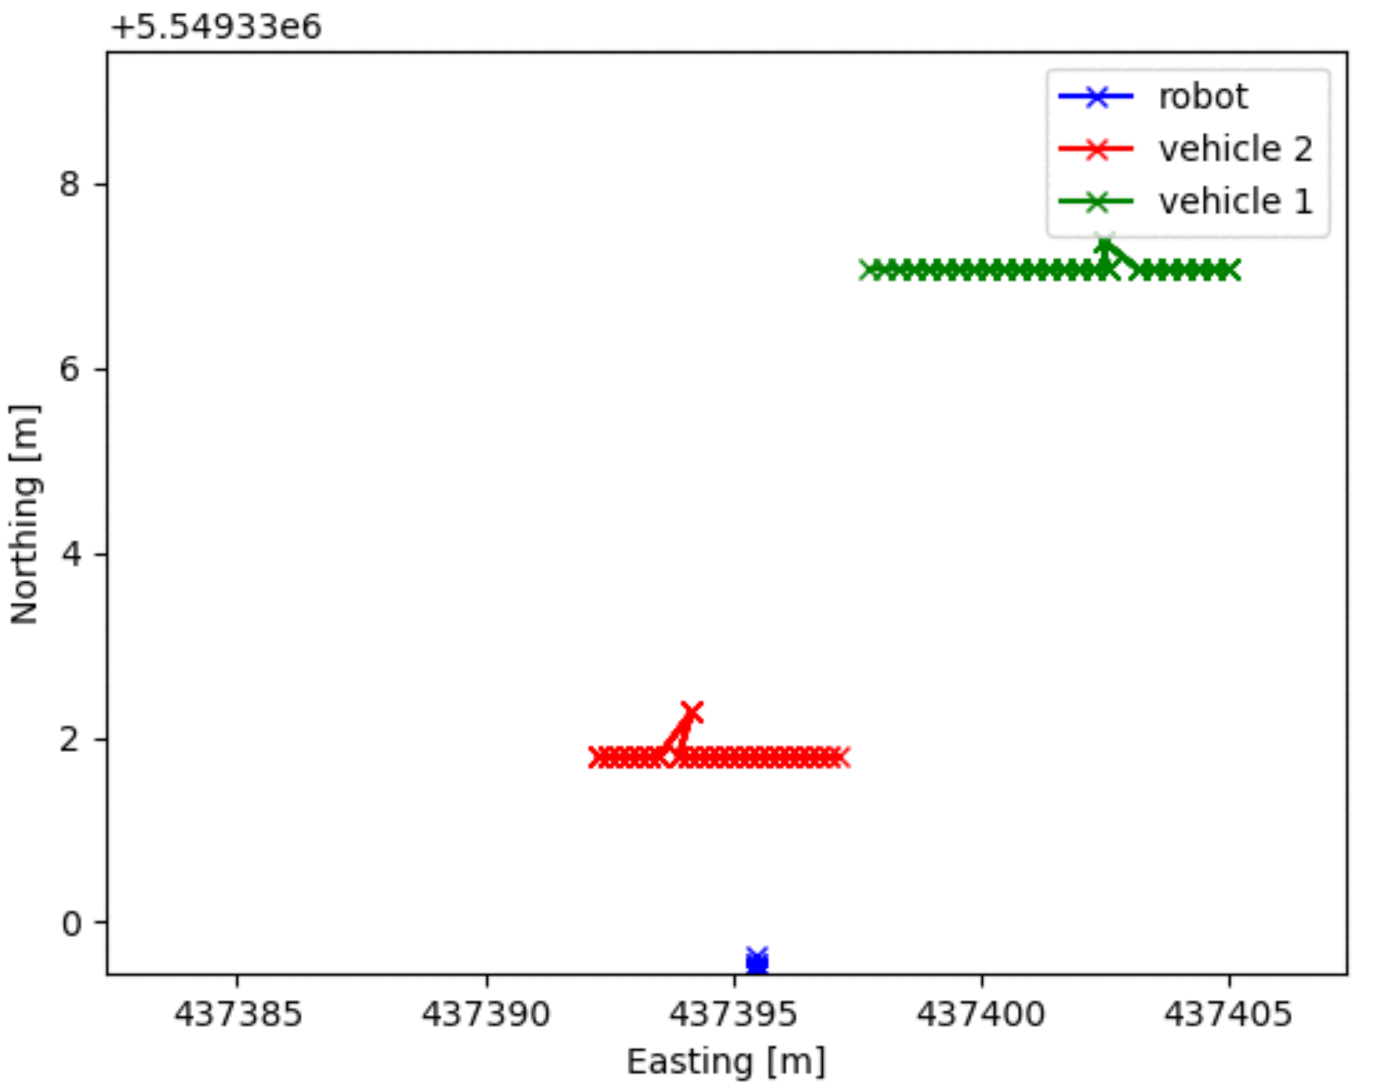
\includegraphics[width=\linewidth]{images/simulations/start_1.png}
                \caption{Scenario 1.}
            \end{subfigure}
            \begin{subfigure}{0.49\linewidth}
                \centering
                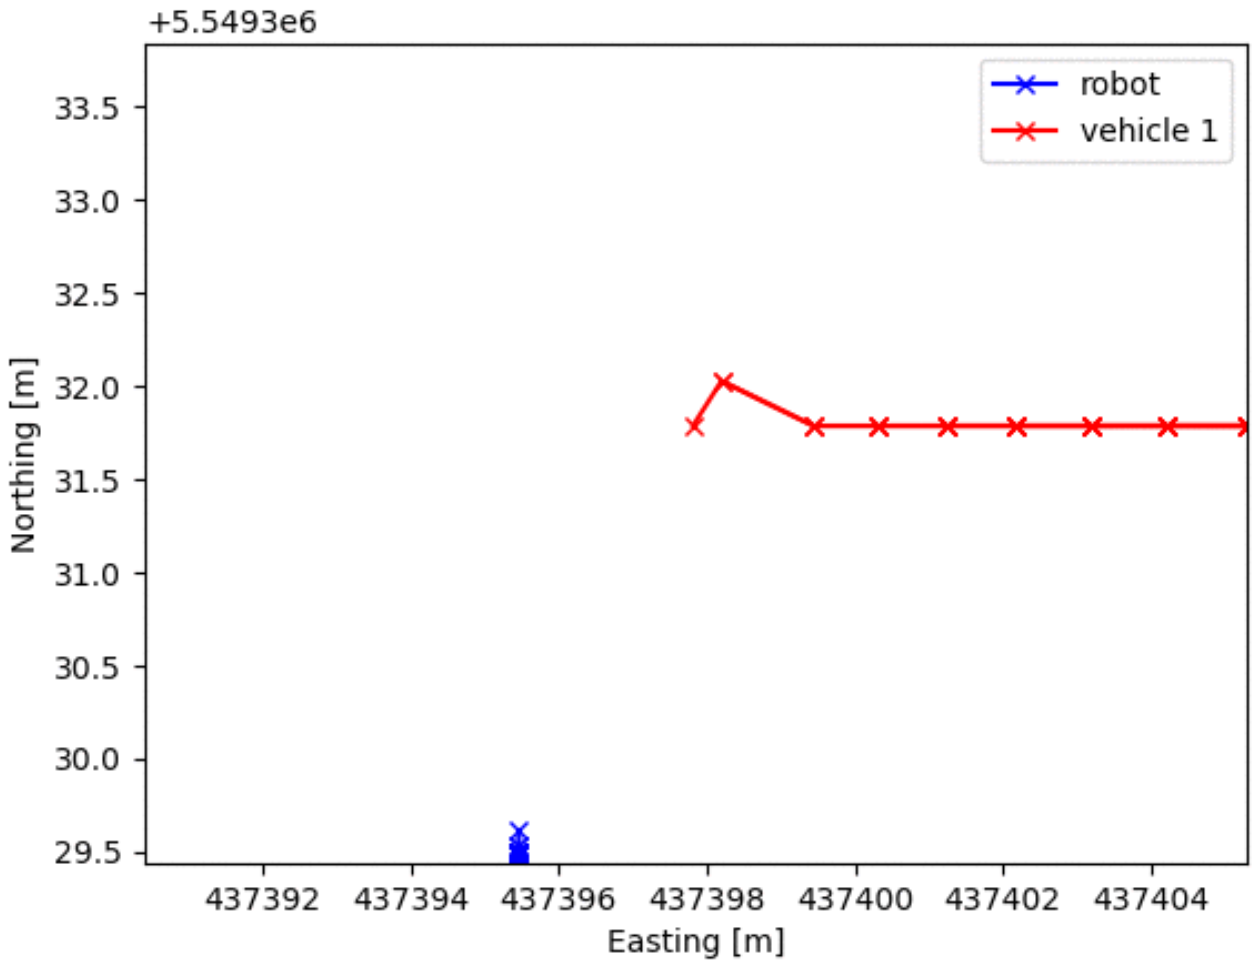
\includegraphics[width=\linewidth]{images/simulations/start_2_2.png}
                \caption{Scenario 2.2.}
            \end{subfigure}
            \begin{subfigure}{0.49\linewidth}
                \centering
                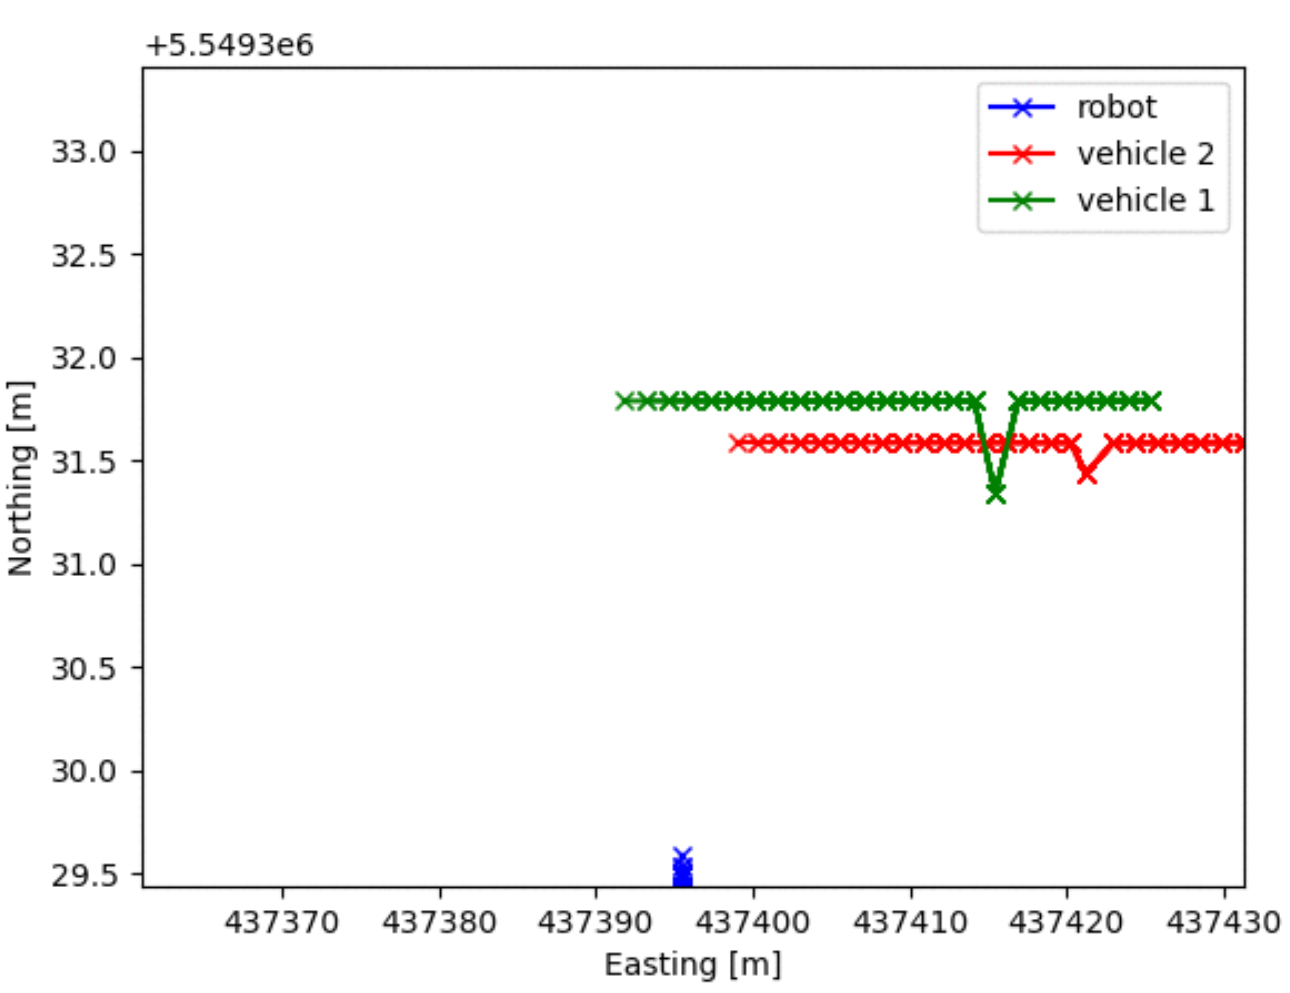
\includegraphics[width=\linewidth]{images/simulations/start_3.png}
                \caption{Scenario 3.}
            \end{subfigure}
            \begin{subfigure}{0.49\linewidth}
                \centering
                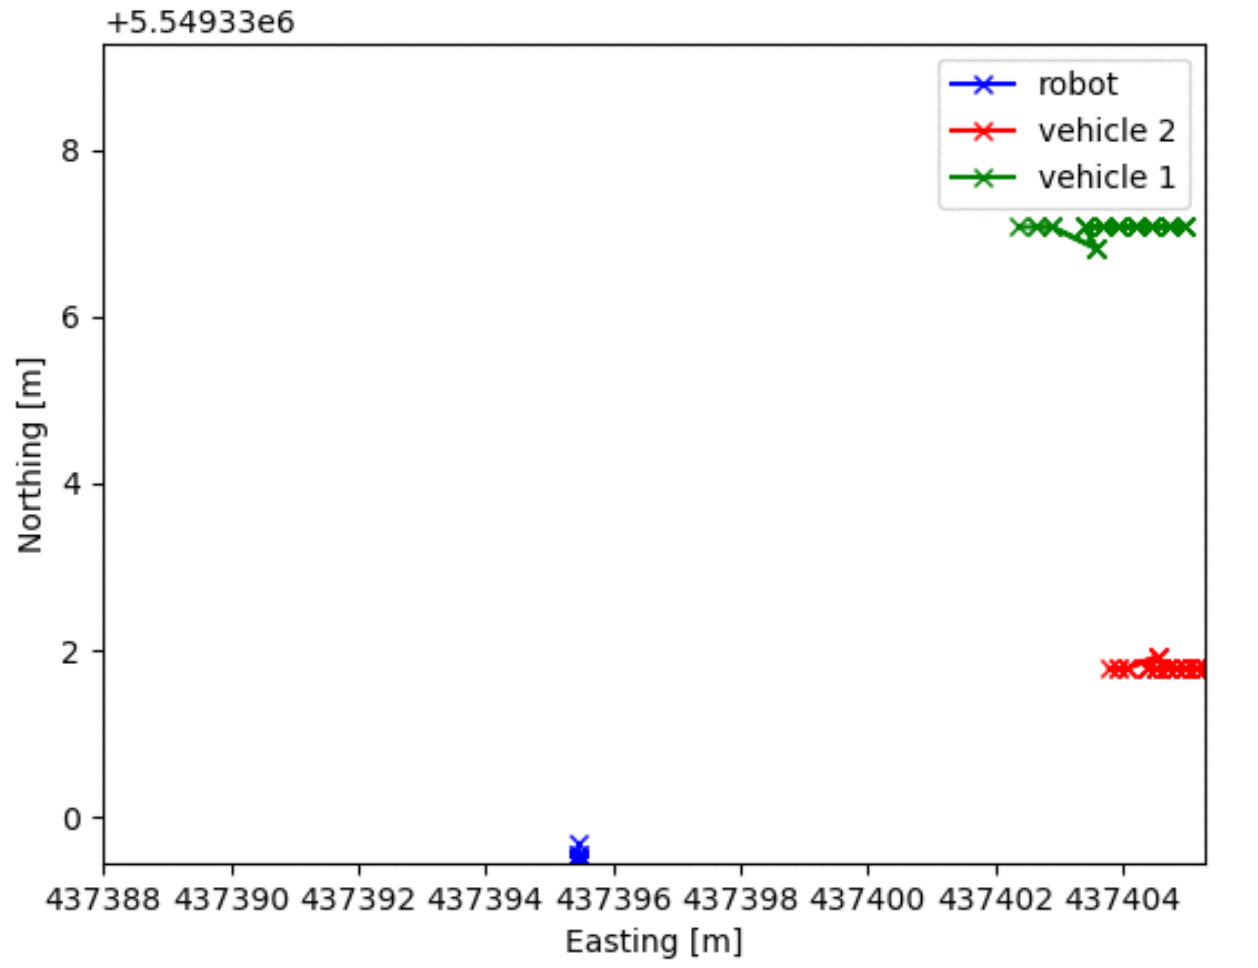
\includegraphics[width=\linewidth]{images/simulations/start_4_1.png}
                \caption{Scenario 4.1.}
            \end{subfigure}
            \begin{subfigure}{0.49\linewidth}
                \centering
                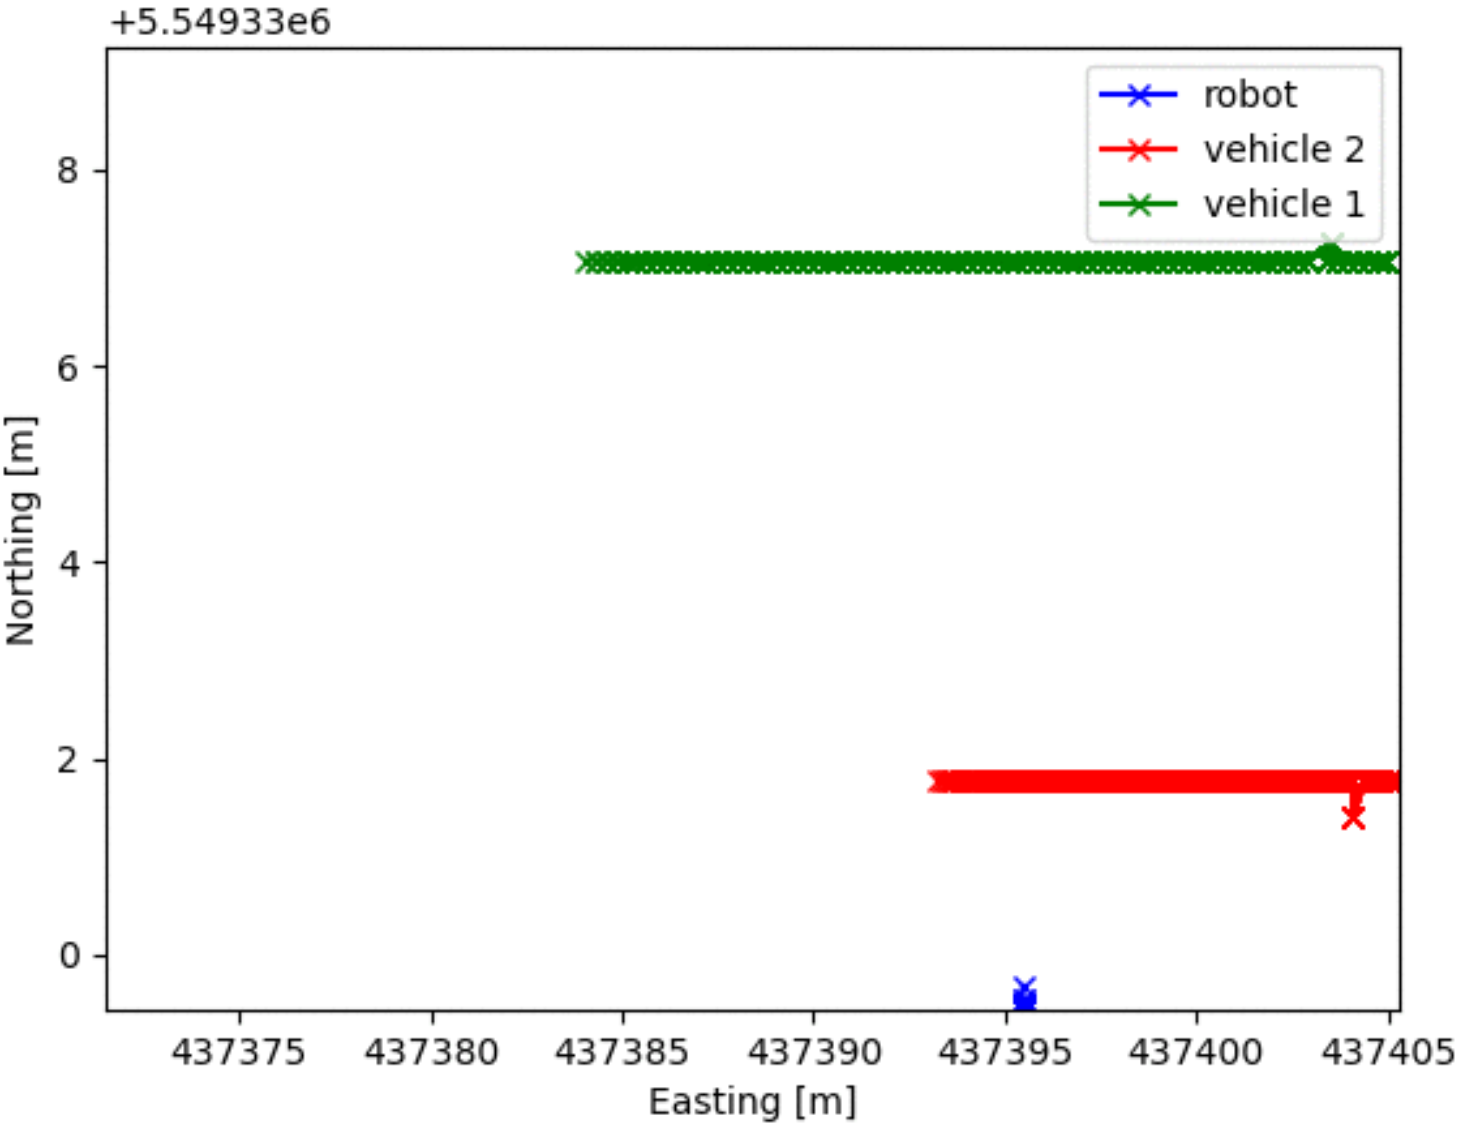
\includegraphics[width=\linewidth]{images/simulations/start_4_2.png}
                \caption{Scenario 4.2.}
            \end{subfigure}
            \begin{subfigure}{0.49\linewidth}
                \centering
                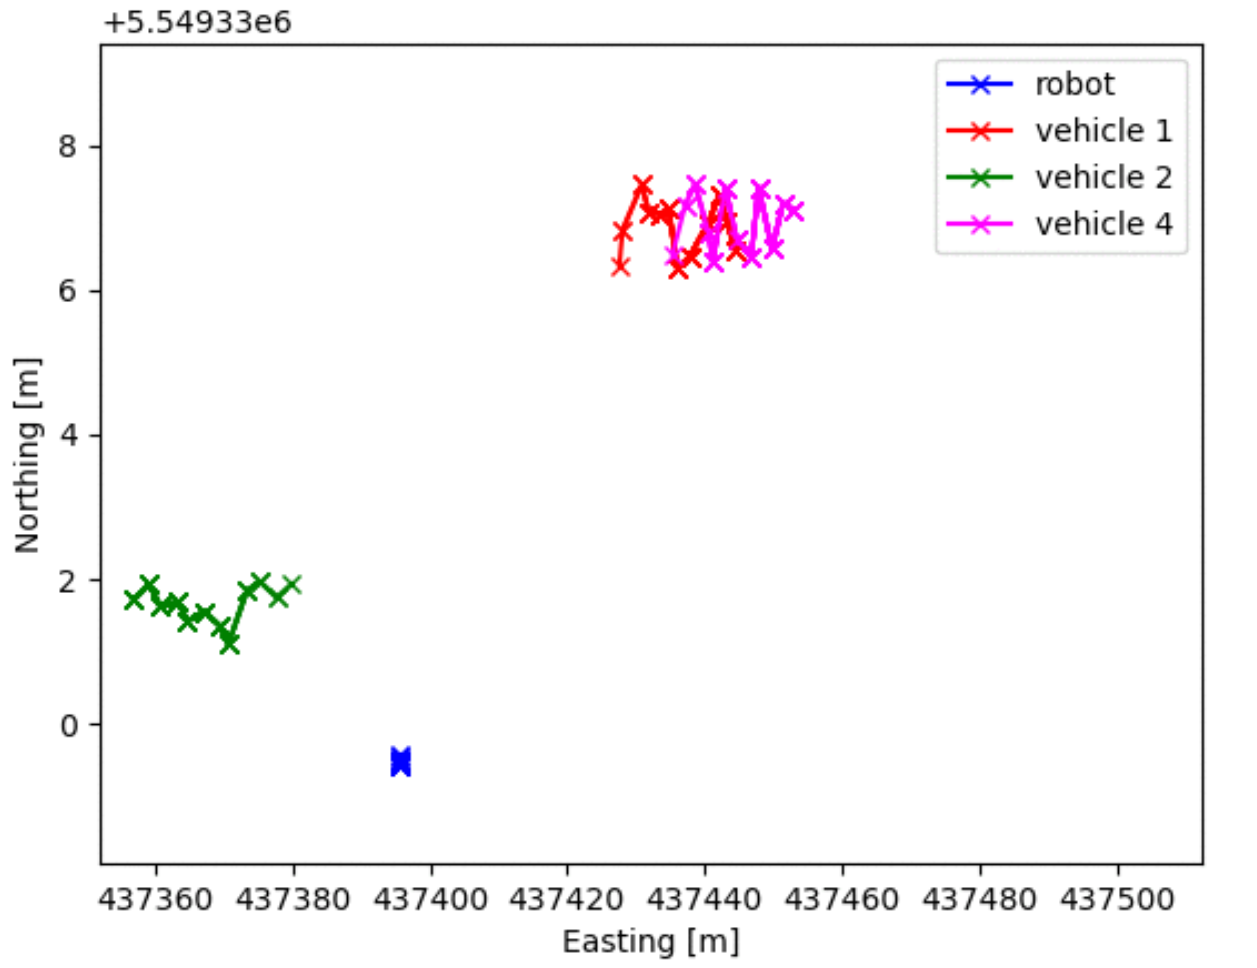
\includegraphics[width=\linewidth]{images/simulations/start_5.png}
                \caption{Scenario 5.}
            \end{subfigure}
            \caption{Start of the robot's movement in the simulation experiments.}
            \label{fig:start}
        \end{figure}
        \newpage
        \thispagestyle{nopagenum}
        \begin{figure}[H]
            \centering
            \begin{subfigure}{0.49\linewidth}
                \centering
                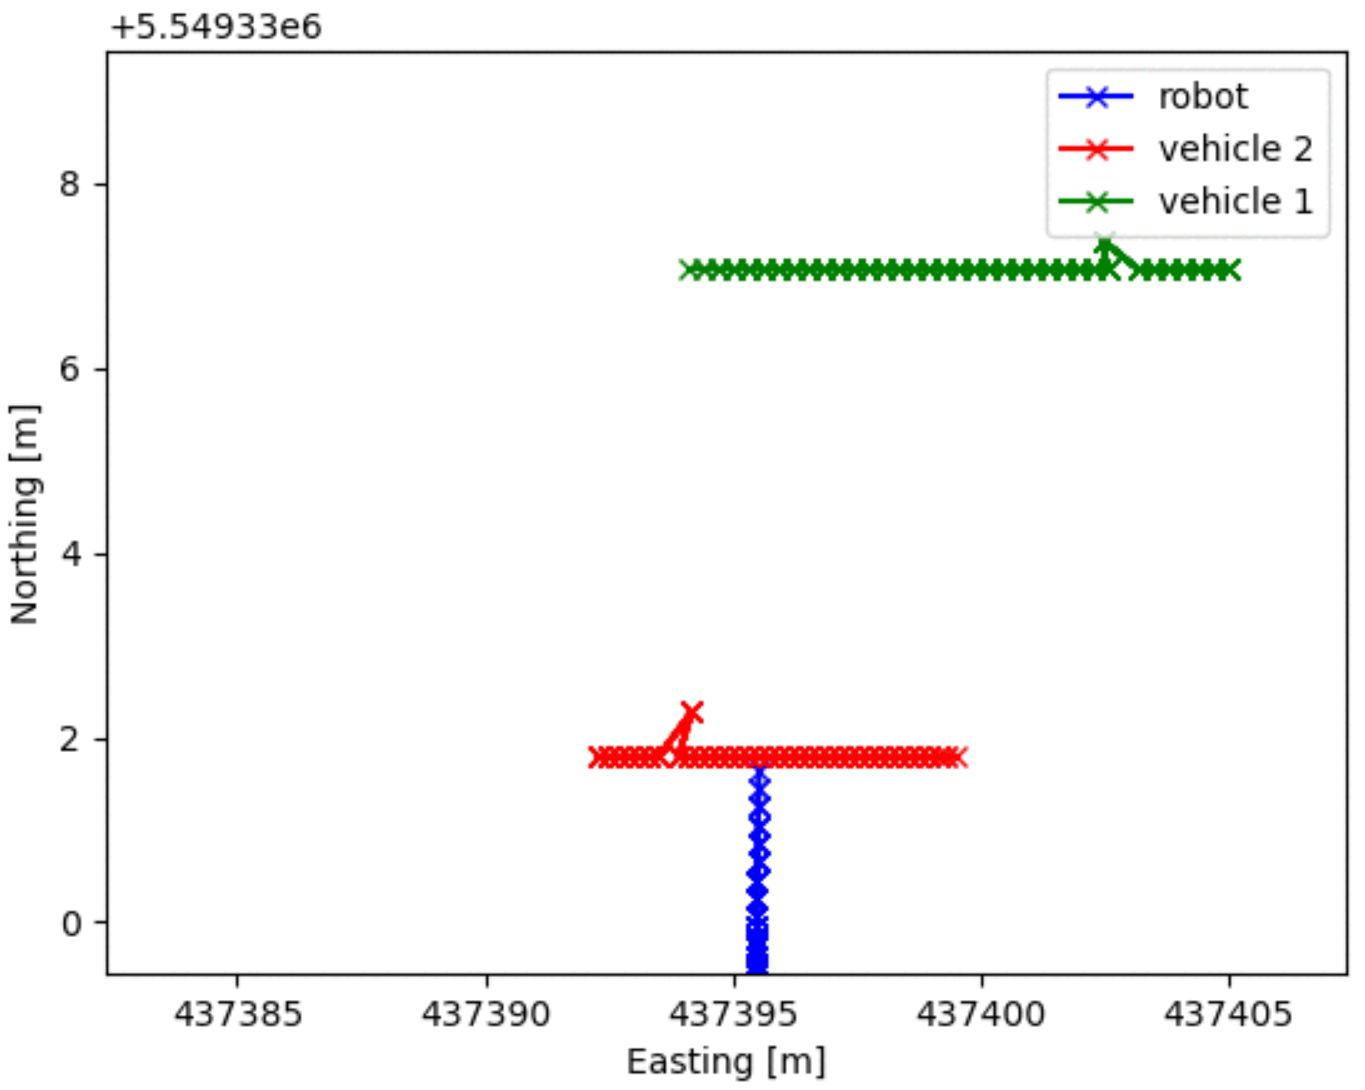
\includegraphics[width=\linewidth]{images/simulations/closest_1.png}
                \caption{Scenario 1.}
            \end{subfigure}
            \begin{subfigure}{0.49\linewidth}
                \centering
                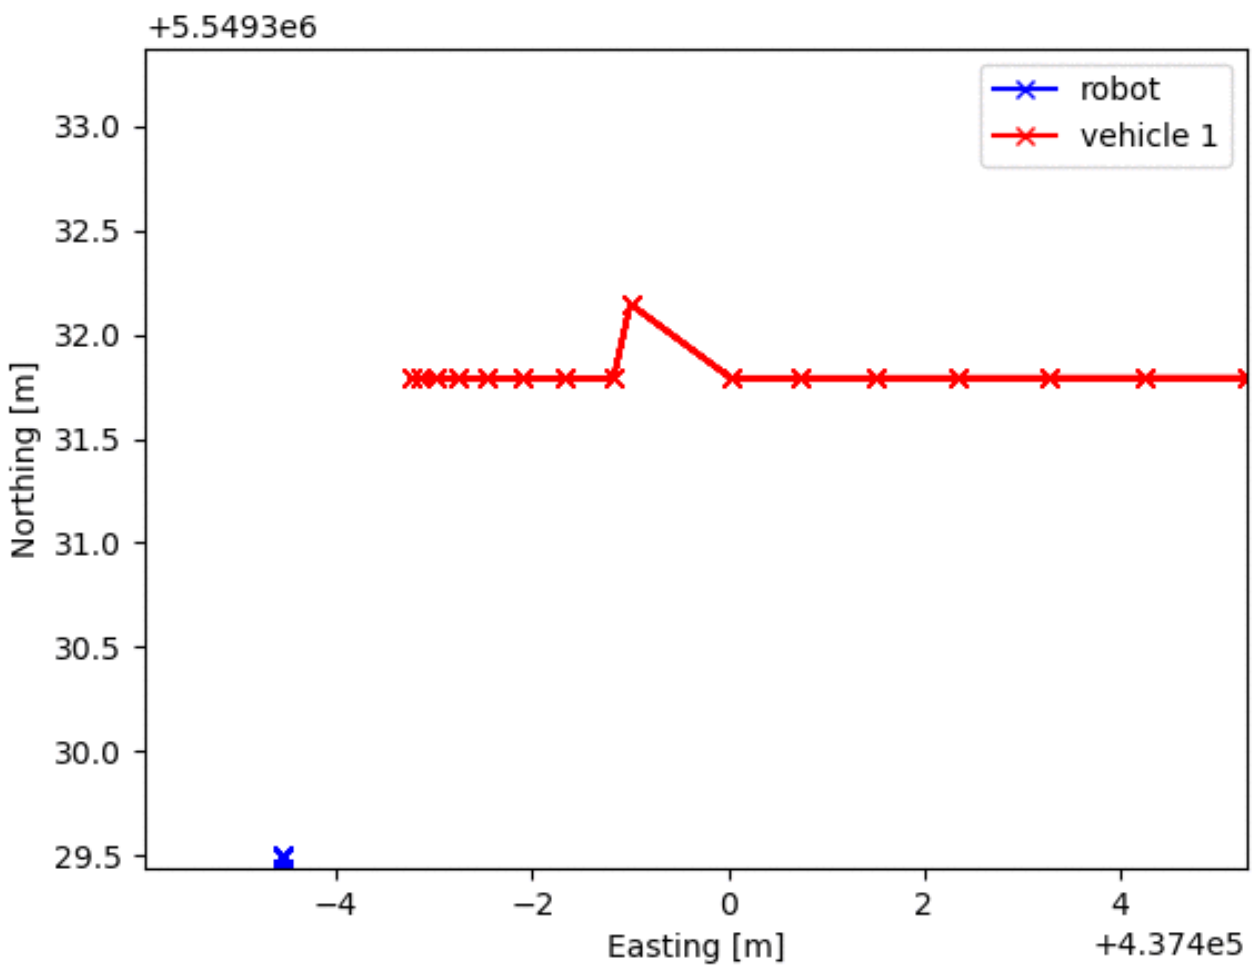
\includegraphics[width=\linewidth]{images/simulations/closest_2_1.png}
                \caption{Scenario 2.1.}
            \end{subfigure}
            \begin{subfigure}{0.49\linewidth}
                \centering
                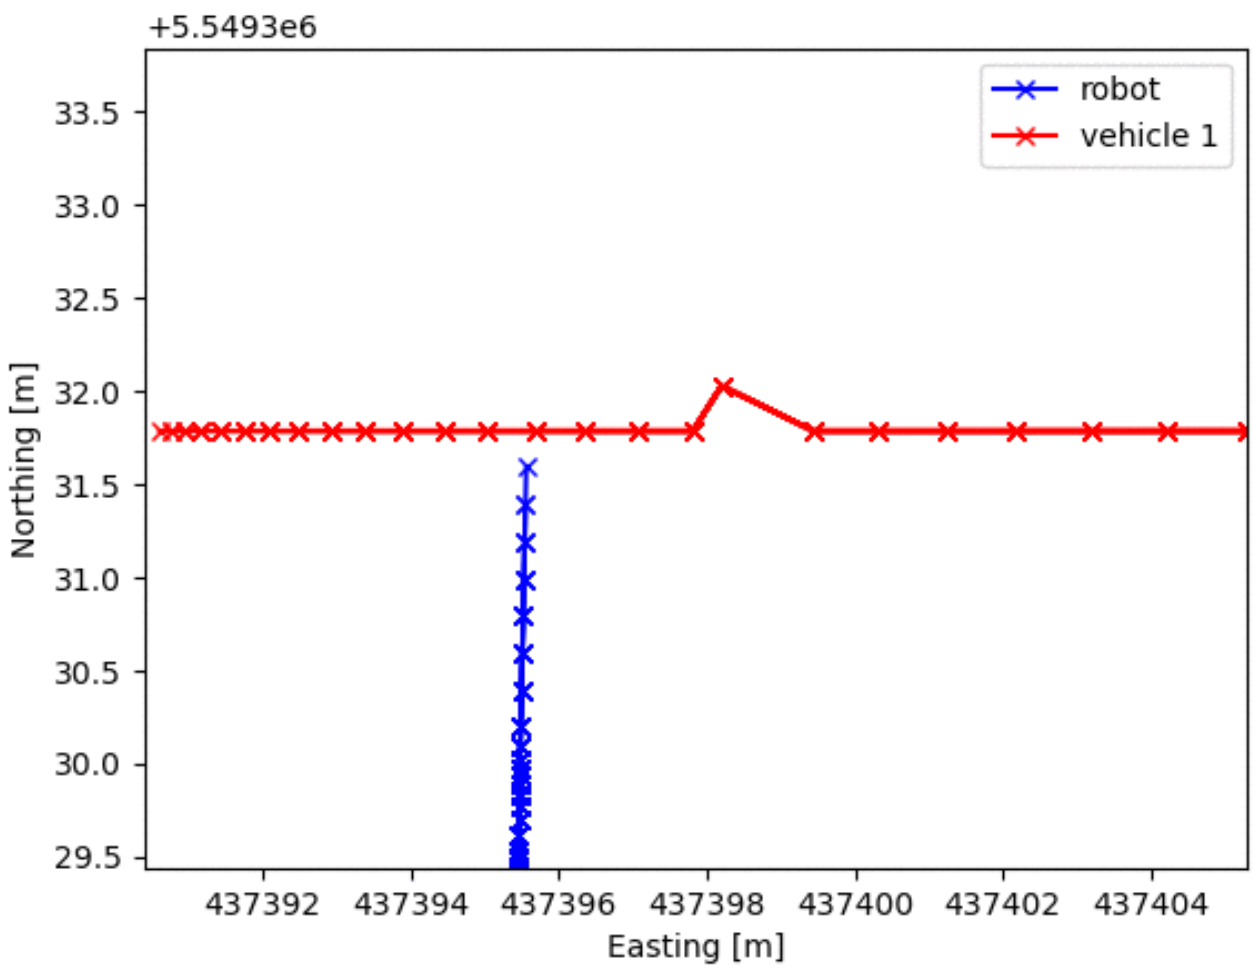
\includegraphics[width=\linewidth]{images/simulations/closest_2_2.png}
                \caption{Scenario 2.2.}
            \end{subfigure}
            \begin{subfigure}{0.49\linewidth}
                \centering
                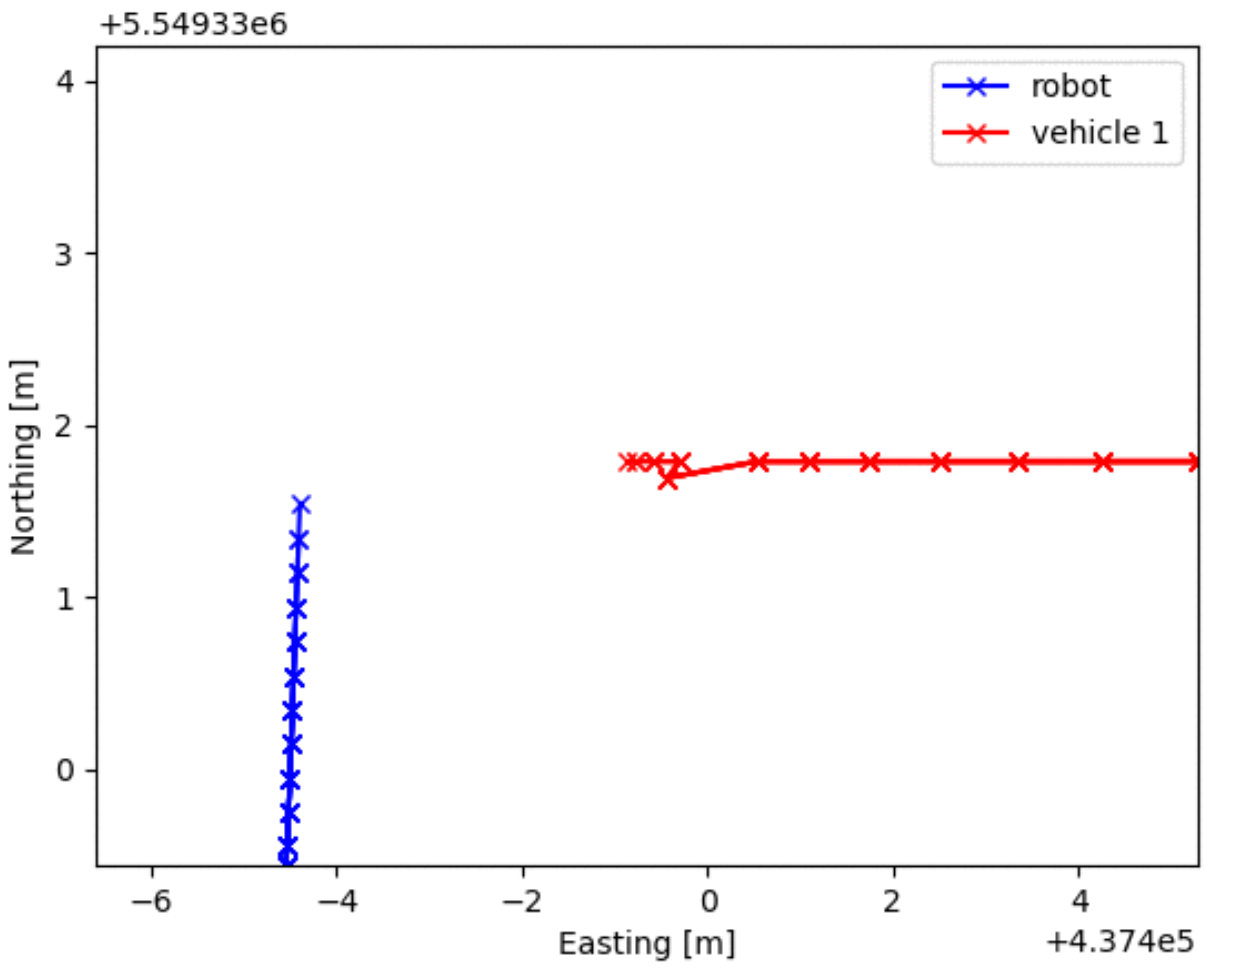
\includegraphics[width=\linewidth]{images/simulations/closest_2_3.png}
                \caption{Scenario 2.3.}
            \end{subfigure}
            \begin{subfigure}{0.49\linewidth}
                \centering
                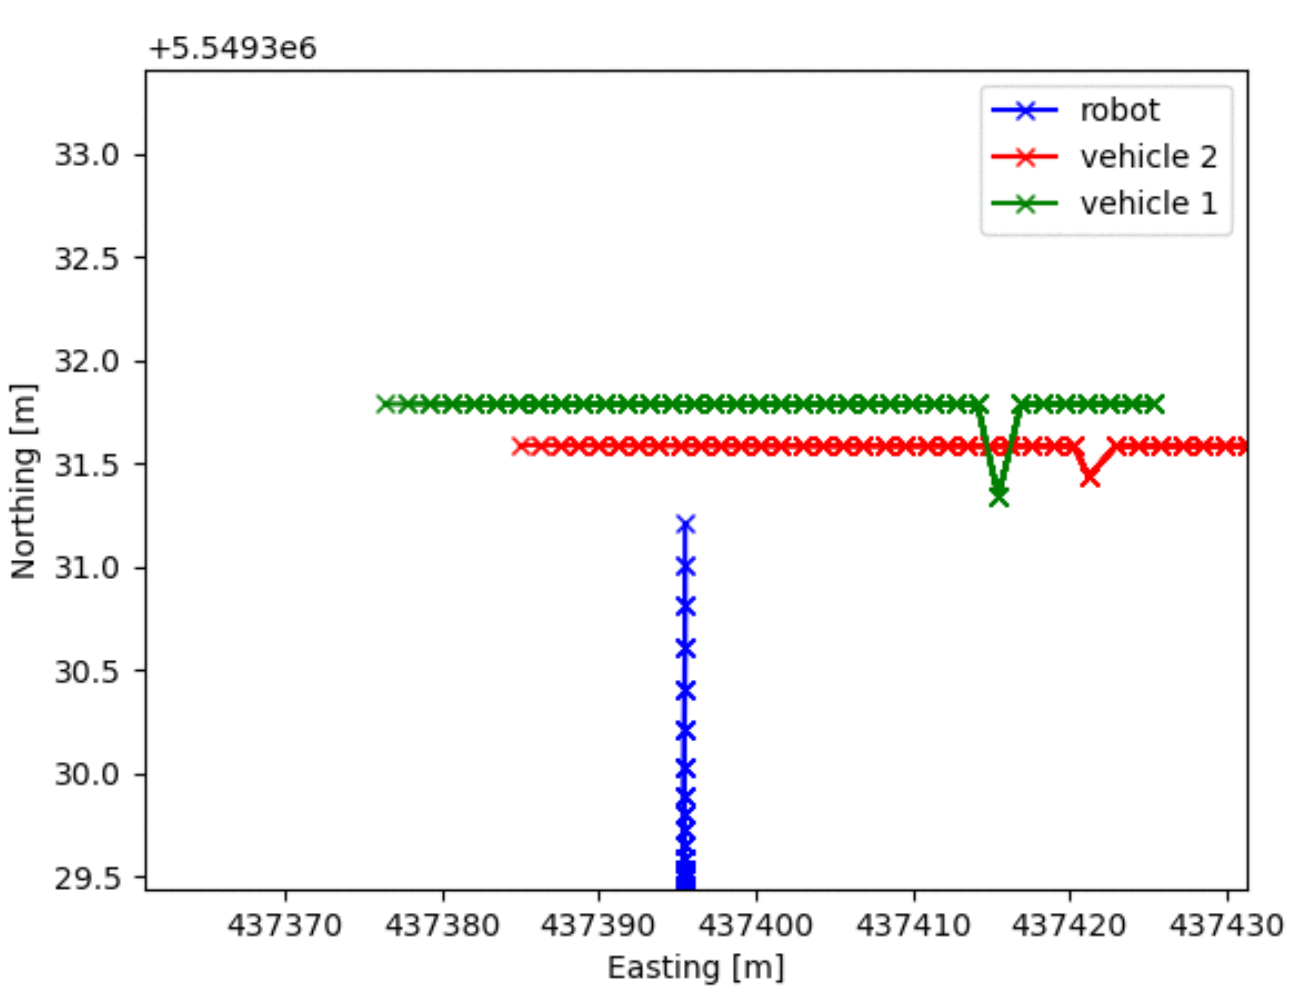
\includegraphics[width=\linewidth]{images/simulations/closest_3.png}
                \caption{Scenario 3.}
            \end{subfigure}
            \begin{subfigure}{0.49\linewidth}
                \centering
                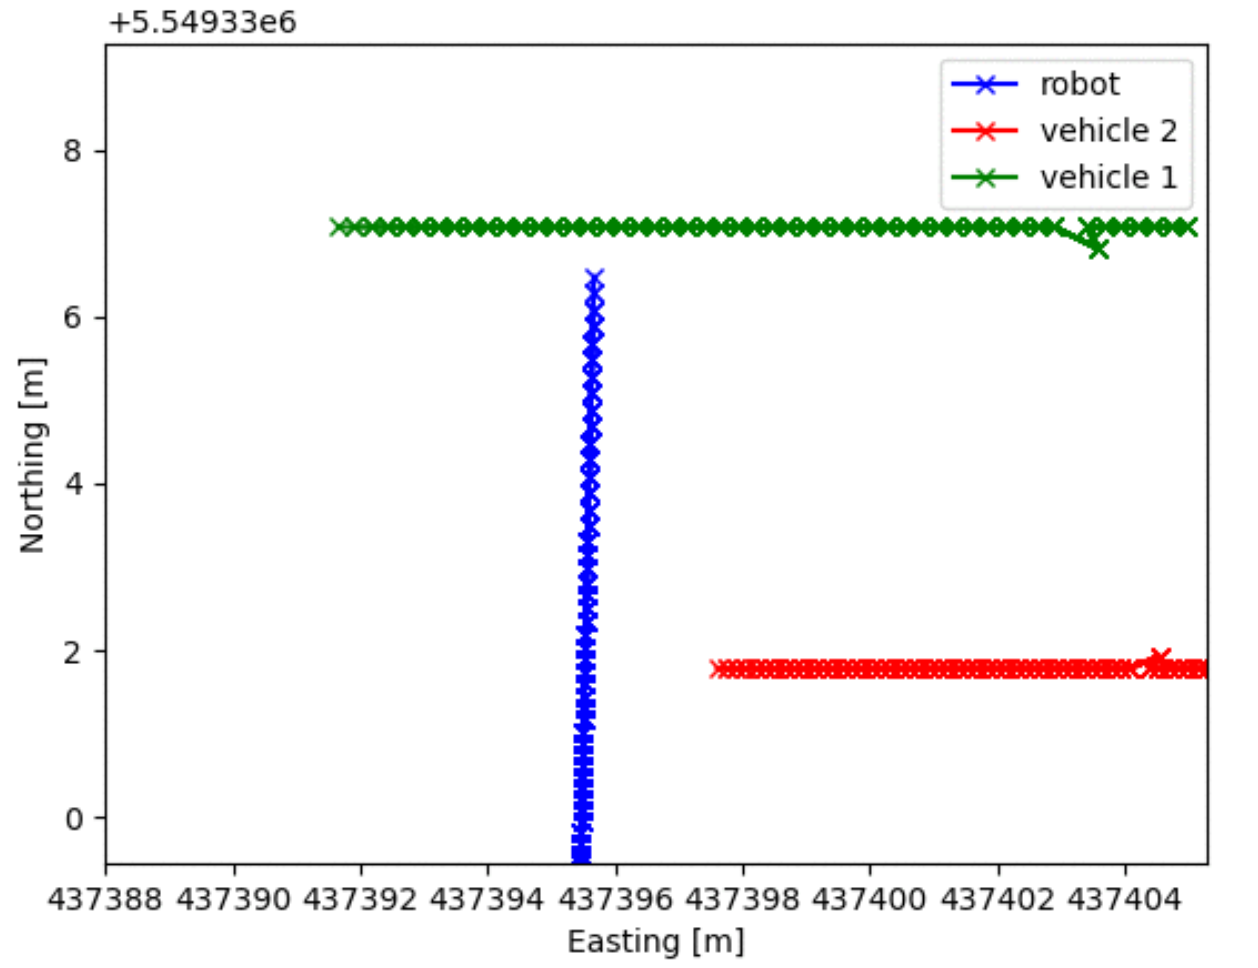
\includegraphics[width=\linewidth]{images/simulations/closest_4_1.png}
                \caption{Scenario 4.1.}
            \end{subfigure}
            \begin{subfigure}{0.49\linewidth}
                \centering
                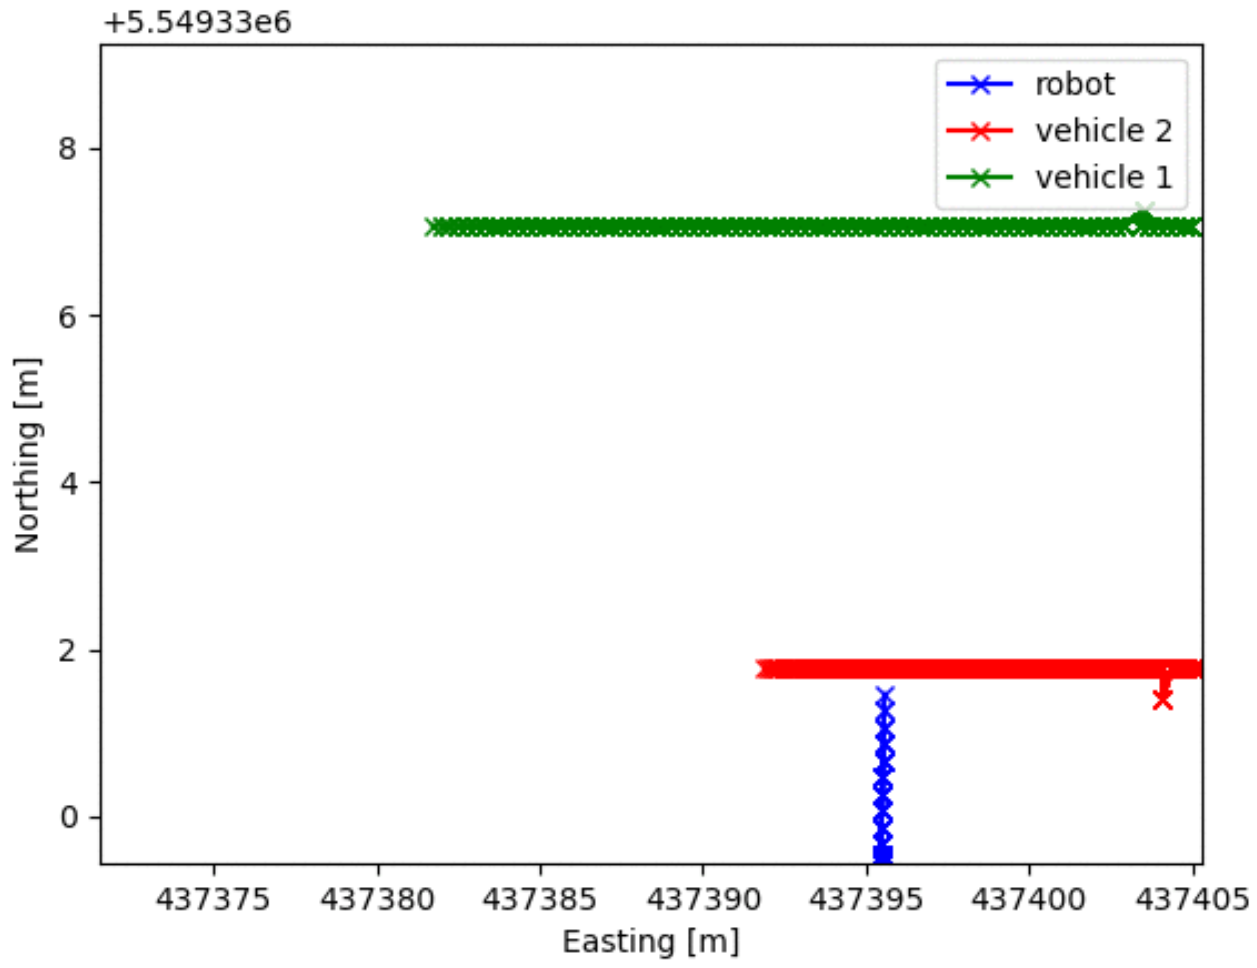
\includegraphics[width=\linewidth]{images/simulations/closest_4_2.png}
                \caption{Scenario 4.2.}
            \end{subfigure}
            \begin{subfigure}{0.49\linewidth}
                \centering
                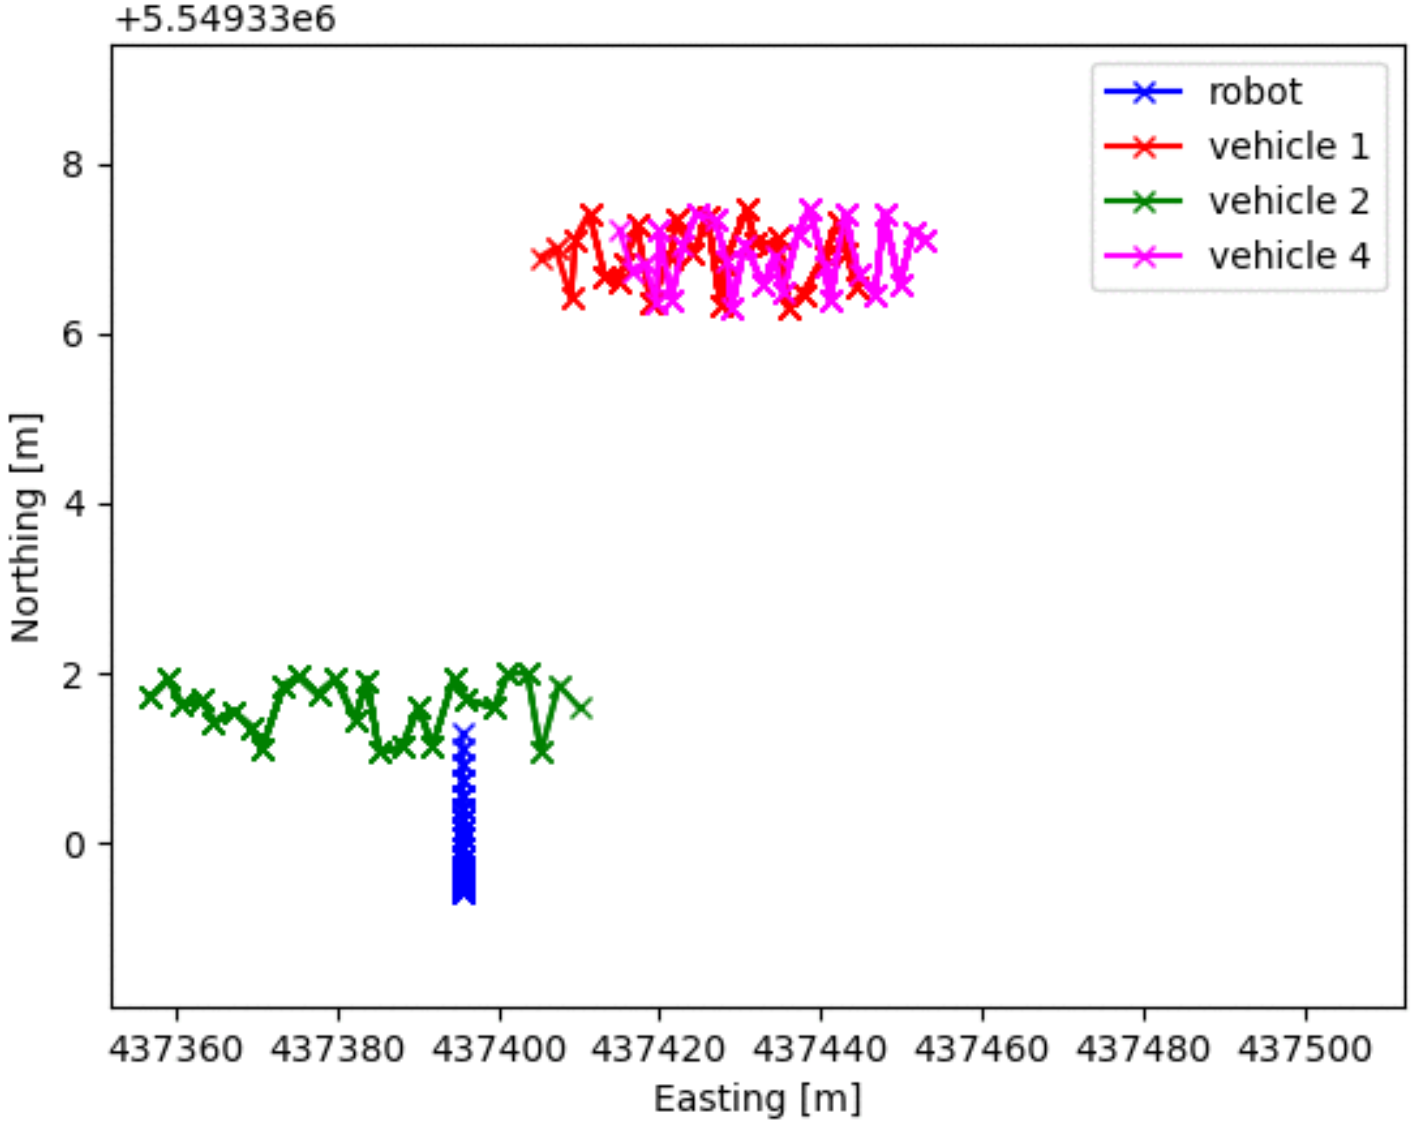
\includegraphics[width=\linewidth]{images/simulations/closest_5.png}
                \caption{Scenario 5.}
            \end{subfigure}
            \caption{The places of the minimal distance between the robot and vehicle in the simulation experiments.}
            \label{fig:closest}
        \end{figure}
